\chapter{The \textsc{Roopl\texttt{++}} Language}
\label{chp:rooplpp}
With the design and implementation of the \textsc{Reversible Object-Oriented Programming Language} (\textsc{Roopl}) and the work-in-progress report of \textsc{Joule}, the first steps into the uncharted lands of Object-Oriented Programming (OOP) and reversibility were taken. In this chapter, we present \rooplpp, the natural successor to \textsc{Roopl}, improving the object instantiation of the language by letting objects live outside \textbf{construct}/\textbf{deconstruct} blocks, allowing complex, reversible programs to be written using OOP methodologies. As with its predecessor, \rooplpp is purely reversible and each component of a program written in \rooplpp is locally invertible. This ensures no computation history is required, nor added program size for backwards program execution.

Inspired by other language successors such as \textsc{C\texttt{++}} was to \textsc{C}, \rooplpp is a superset of \textsc{Roopl}, containing all original functionality of its predecessor, extended with new object instantiation methods for increased programming usability and an array type.

\vskip 2em

\begin{figure}[ht]
    \centering
    \lstinputlisting[language=roopl, style=basic, frame=none, multicols=2]{fib.rplpp}
    \caption{Example \rooplpp program implementing the Fibonacci function}    
\end{figure}
\newpage


\section{Syntax}
\label{sec:syntax}
A \rooplpp program consists, analogously to a \textsc{Roopl} program, of one or more class definitions, each with a varying number of fields and class methods. The entry point of the program is a nullary main method, which is defined exactly once and is instantiated during program start-up. Fields of the main object will serve as output of the program, just as in \textsc{Roopl}.
\begin{figure}[h]
    \centering
    \vspace{3mm}
    \textbf{\rooplpp Grammar}
    \begin{align}
    prog		\quad&::= \quad cl^+ \tag{program}\\
    cl			\quad&::=\quad \textbf{class}\ c\ (\textbf{inherits}\ c)^?\ (t\ x)^*\ m^+\tag{class definition}\\
    d           \quad&::=\quad c\ |\ c[e]\ |\ \textbf{int}[e] \tag{class and arrays}\\
    t			\quad&::=\quad \textbf{int}\ |\ c\ |\ \textbf{int}[]\ |\ c[]\tag{data type}\\
    y          \quad&::=\quad x\ |\ x[e] \tag{variable identifiers}\\
    m			\quad&::=\quad \textbf{method}\ q\textbf{\texttt{(}}t\ x,\ \dots,\ t\ x\textbf{\texttt{)}}\ s\tag{method}\\
    s			\quad&::=\quad y\ \odot\textbf{\texttt{=}}\ e\ |\ y\ \textbf{\texttt{<=>}}\ y\tag{assignment}\\\
    			&\ |\ \qquad \textbf{if}\ e\ \textbf{then}\ s\ \textbf{else}\ s\ \textbf{fi}\ e\tag{conditional}\\
    			&\ |\ \qquad \textbf{from}\ e\ \textbf{do}\ s\ \textbf{loop}\ s\ \textbf{until}\ e\tag{loop}\\
                &\ |\ \qquad \textbf{construct}\ c\ x\quad s\quad\textbf{destruct}\ x\tag{object block}\\
                &\ |\ \qquad \textbf{local}\ t\ x\ \texttt{=}\ e\quad s\quad\textbf{delocal}\ t\ x\ \texttt{=}\ e\tag{local variable block}\\
                &\ |\ \qquad \textbf{new}\ d\ y\ |\ \textbf{delete}\ d\ y \tag{object con- and destruction}\\
                &\ |\ \qquad \textbf{copy}\ d\ y\ y\ |\ \textbf{uncopy}\ d\ y\ y \tag{reference con- and destruction}\\
    			&\ |\ \qquad \textbf{call}\ q\textbf{\texttt{(}}x,\ \dots,\ x\textbf{\texttt{)}}\ |\ \textbf{uncall}\ q\textbf{\texttt{(}}x,\ \dots,\ x\textbf{\texttt{)}}\tag{local method invocation}\\
    			&\ |\ \qquad \textbf{call}\ y\textbf{\texttt{::}}q\textbf{\texttt{(}}x,\ \dots,\ x\textbf{\texttt{)}}\ |\ \textbf{uncall}\ y\textbf{\texttt{::}}q\textbf{\texttt{(}}x,\ \dots,\ x\textbf{\texttt{)}}\tag{method invocation}\\
    			&\ |\ \qquad \textbf{skip}\ |\ s\ s\tag{statement sequence}\\
    e			\quad&::=\quad \overline{n}\ |\ x\ |\ x[e]\ |\ \textbf{\texttt{nil}}\ |\ e\ \otimes\ e\tag{expression}\\
    \odot	\quad&::=\quad \textbf{\texttt{+}}\ |\ \textbf{\texttt{-}}\ |\ \textbf{\texttt{\^}}\tag{operator}\\
    \otimes\quad&::=\quad \odot\ |\ \textbf{\texttt{*}}\ |\ \textbf{\texttt{/}}\ |\ \textbf{\texttt{\%}}\ |\ \textbf{\texttt{\&}}\ |\ \textbf{\texttt{|}}\ |\ \textbf{\texttt{\&\&}}\ |\ \textbf{\texttt{||}}\ |\ \textbf{\texttt{<}}\ |\ \textbf{\texttt{\textgreater}}\ |\ \textbf{\texttt{=}}\ |\ \textbf{\texttt{!=}}\ |\ \textbf{\texttt{<=}}\ |\ \textbf{\texttt{\textgreater=}}\tag{operator}
    \end{align}
    \vspace{2mm}
    \textbf{Syntax Domains}
    \begin{align*}
    prog &\in \text{Programs} & s &\in \text{Statements}      & n &\in \text{Constants} \\
    cl   &\in \text{Classes}  & e &\in \text{Expressions}     & x &\in \text{VarIDs}    \\
    t    &\in \text{Types}    & \odot &\in \text{ModOps}      & q &\in \text{MethodIDs} \\
    m    &\in \text{Methods}  & \otimes &\in \text{Operators} & c &\in \text{ClassIDs}
    \end{align*}
    \caption{Syntax domains and EBNF grammar for \rooplpp}
    \label{fig:roopl-grammar}
\end{figure}

The \rooplpp grammar extends the grammar of \textsc{Roopl}  with a new static integer or class array type and a new object lifetime option in form of objects outside of blocks, using the \textbf{new} and \textbf{delete} approach. Furthermore, the local block extension proposed in~\cite{th:roopl} has become a standard part of the language. Class definitions remains unchanged, and consists of a \textbf{class} keyword followed by a class name. Subclasses must be specified using the \textbf{inherits} keyword and a following parent class name. Classes can have any number of fields of any of the data types, including the new Array type. A class definition is required to include at least one method, defined by the \textbf{method} keyword followed by a method name, a comma-separated list of parameters and a body.

Reversible assignments for integer variables and integer array elements uses similar syntax as \textsc{Janus} assignments, by updating a variable through any of the addition (\texttt{+=}), subtraction (\texttt{-=}) or bitwise XOR (\texttt{\^{}=}) operators. As with \textsc{Janus}, when updating a variable $x$ using any of said operators, the right-hand side of the operator argument must be entirely independent of $x$ to maintain reversibility. Usage of these reversible assignment operators for object or array variables is undefined. Variables and array elements of any type can be swapped using the \texttt{<=>} operator as long as the variable is of same type as the array type. If an array is of a base class type, subclass variable values can be swapped in and out of the array, as long as the resulting value in the variable is still of the original subclass type.  

\rooplpp objects can be instantiated in two ways. Either using object blocks known from \textsc{Roopl}, or by using the \textbf{new} statement. The object-blocks have a statically-scoped lifetime, as the object only exists within the \textbf{construct} and \textbf{destruct} segments. Using \textbf{new} allows the object to live until program termination, if the program terminates with a \textbf{delete} call. By design, it is the programmers responsibility to deallocate objects instantiated by the \textbf{new} statement.

Arrays are also instantiated by usage of \textbf{new} and \textbf{delete}. Assignment of array cells depend on the type of the arrays, which is further discussed in section~\ref{sec:array-instantiation}.

The methodologies for argument aliasing and its restrictions on method on invocations from \textsc{Roopl} carries over in \rooplpp and object fields are as such disallowed as arguments to local methods to prevent irreversible updates and non-local method calls to a passed objects are prohibited. The parameter passing scheme remains call-by-reference and the object model of \textsc{Roopl} remains largely unchanged in \rooplpp.

\section{Object Instantiation}
\label{sec:object-instantiation}
Object instantiation through the \textbf{new} statement follows the pattern of the mechanics known from the \textbf{construct}/\textbf{destruct} blocks from \textsc{Roopl}, but providing improved scoping and lifetime options objects. The mechanisms of the statement 

\begin{align*}
\textbf{construct}\ c\ x\ \quad s\ \quad \textbf{destruct}\ x
\end{align*}

are as follows:

\begin{enumerate}
\item Memory for an object of class $c$ is allocated. All fields are automatically zero-initialized by virtue of residing in already zero-cleared memory.
\item The block statement $s$ is executed, with the name $x$ representing a reference to the newly allocated object.
\item The reference $x$ may be modified by swapping its value with that of other references of the same type, but it should be restored to its original value within the statement block $s$, otherwise the meaning of the object block is undefined.
\item Any state that is accumulated within the object should be cleared or uncomputed before the end of the statement is reached, otherwise the meaning of the object block is undefined.
\item The zero-cleared memory is reclaimed by the system.
\end{enumerate}

The statement pair consisting of

\begin{align*}
\textbf{new}\ c\ x\ \quad \dots\ \quad \textbf{delete}\ c\ x\
\end{align*}

could be considered a \textit{dynamic} block, meaning we can have overlapping blocks. Compared to \textbf{construct}/\textbf{destruct} block consisting of a single statement, the \textbf{new}/\textbf{delete} block consist of two separate statements. We can as such initialize an object $x$ of class $c$ and an object $y$ of class $d$ and destroy $x$ before we destroy $y$, a feature that was not possible in \textsc{Roopl}. The mechanisms of the \textbf{new} statement are as follows:

\begin{enumerate}
    \item Memory for an object of class $c$ is allocated. All fields are automatically zero-initialized by virtue of residing in already zero-cleared memory.
    \item The address of the newly allocated block is stored in the previously defined and zero-cleared reference $x$.
\end{enumerate}

and the mechanisms of the \textbf{delete} statement are as follow

\begin{enumerate}
    \item The reference $x$ may be modified by swapping its internal field values with that of other references of the same type, but should be zero-cleared before a \textbf{delete} statement is called on $x$, otherwise the meaning of the object deletion is undefined.
    \item Any state that is accumulated within the object should be cleared or uncomputed before the \textbf{delete} statement is executed, otherwise the meaning of the object block is undefined.
    \item The zero-cleared memory is reclaimed by the system.
\end{enumerate}

The mechanisms of the \textbf{new} and \textbf{delete} statements are, essentially, a split of the mechanisms of the \textbf{construct}/\textbf{destruct} blocks into two separate statements. As with \textsc{Roopl}, fields must be zero-cleared after object deletion, otherwise it is impossible for the system to reclaim the memory reversibly. This is the responsibility of the of the programmer to maintain this, and to ensure that objects are indeed deleted in the first place. A \textbf{new} statement without a corresponding \textbf{delete} statement targeting the same object further ahead in the program is undefined, as is a delete statement without a preceding \textbf{new} statement.

Note that variable scopes are always static, but object scopes can be either static (using \textbf{construct}/\textbf{destruct}) or dynamic (using \textbf{new}/\textbf{delete}).
\newpage

\section{Array Model}
\label{sec:array-model}
Besides asymmetric object lifetimes, \rooplpp also introduces reversible, fixed-sized arrays of either integer or object types. While \textsc{Roopl} only featured integers and custom data types in form of classes, one of its main inspirations, \textsc{Janus}, implemented static, reversible arrays~\cite{ty:janus}. 

While \textsc{Roopl} by design did not include any data storage language constructs, as they are not especially noteworthy nor interesting from an OOP perspective, they do generally improve the expressiveness of the language. Arrays were decided to be part of the core language for this reason, as one of the main goals of \rooplpp is increased expressiveness while implementing reversible programs.

In \rooplpp, arrays expand upon the array model from \textsc{Janus}. Arrays are indexed by integers, starting from 0. In \textsc{Janus}, only integer arrays were allowed, while in \rooplpp arrays of any type can be defined, meaning either integer arrays or custom data types in form of class arrays. They are however, still restricted to one dimension.

Array element accessing is accomplished using the bracket notation known from \textsc{Janus}. Accessing an out-of-bounds index is undefined.
Array instantiation and element assignments, aliasing and circularity is described in detail in the following section.

Arrays can contain elements of different classes sharing a base class, that is, say class $A$ and $B$ both inherit from some class $C$ and array $x$ is of type $C[]$. In this case, the array can hold elements of type $A$, $B$, and $C$. When swapping array elements from a base class array with object references, the programmer must be careful not to swap the values of, say, and $A$ object into a $B$ reference.

\section{Array Instantiation}
\label{sec:array-instantiation}
Array instantiation uses the \textbf{new} and \textbf{delete} keywords to reversibly construct and destruct array types. The mechanisms of the statement
\begin{align*}
\textbf{new}\ \textbf{int}[e]\ x
\end{align*} 
in which we reserve memory for an integer array are as follows

\begin{enumerate}
    \item The expression $e$ is evaluated
    \item Memory equal to the integer value that $e$ evaluates to and an additional small amount of memory for of overhead is reserved for the array.
    \item The address of the newly allocated memory is stored in the previously defined and zero-cleared reference $x$.
\end{enumerate}

In \rooplpp, we only allow instantiation of fixed-sized arrays of a length defined in the given expression $e$. Array elements are assigned dependent on the type of the array. For integer arrays, any of the reversible assignment operators can be used to assign values to cells. For class arrays, we assign cell elements a little differently. We either make use of the \textbf{new} and \textbf{delete} statements, but instead of specifying which variable should hold the newly created/deleted object or array, we specify which array cell it should be stored in or we use the \textbf{swap} statement to swap values in and out of array cells. Usage of the assignment operators on non-integer arrays is undefined.

\begin{lstlisting}[caption={Assignment of array elements}, language=roopl, style=basic,label={lst:array-assignment}]
    new int[5] intArray         // Init new integer array
    new Foo[2] fooArray         // init new Foo array

    intArray[1] += 10           // Legal array integer assignment
    intArray[1] -= 10           // Legal Zero-clearing for integer array cells

    new Foo fooObject
    fooArray[0] <=> fooObject   // Legal object array cell assignment
    new Foo fooArray[2]         // Legal object array cell assignment

    ...                         // Clear all array cells

    delete Foo fooArray[0]      // Legal object array cell zero-clearing
    delete Foo fooArray[1]      // Legal object array cell zero-clearing
\end{lstlisting}
 
As with \rooplpp objects instantiated outside of \textbf{construct}/\textbf{destruct} blocks, arrays must be deleted before program termination to reversibly allow the system to reclaim the memory. Before deletion of an array, all its elements must be zero-cleared such that no garbage data resides in memory after erasure of the array reference.

Consider the statement
\begin{align*}
\textbf{delete}\ \textbf{int}[e]\ x
\end{align*}

with the following mechanics

\begin{enumerate}
\item The reference $x$ may be modified by swapping, assigning cell element values and zero-clearing cell element values, but must be restored to an array of same type with fully zero-cleared cells before the \textbf{delete} statement. Otherwise, the meaning of the statement is undefined.
\item The value of the expression $e$ is evaluated and used to reclaim the allocated memory space. 
\item If the reference $x$ is a fully zero-cleared array upon the \textbf{delete} statement execution, the zero-cleared memory is reclaimed by the system.
\end{enumerate}

With reversible, fixed-sized arrays of varying types, we must be extremely careful when updating and assigning values, to ensure we maintain reversibility and avoid irreversible statements. Therefore, when assigning or updating integer elements with one of the reversible assignment operators, we prohibit the cell value from being reference on the right hand side, meaning the following statement is prohibited
\begin{align*}
x[5]\ \texttt{+=}\ x[5] + 1 
\end{align*}

However, we do allow other initialized, non-zero-cleared array elements from the same array or arrays of same type to be referenced in the right hand side of the statement. As with regular assignment, we still prohibit the left side reference to occur in the ride side, meaning the following statements are also prohibited
\begin{align*}
x\ \texttt{+=}\ y[x]\\
y[x]\ \texttt{+=}\ x
\end{align*}

\newpage
\section{Referencing}
\label{sec:referencing-layout}
Besides the addition of dynamically lifetimed objects and arrays, \rooplpp also increases program flexibility by allowing multiple references to objects and arrays through the usage of the \textbf{copy} statement. Once instantiated through either a \textbf{new} or \textbf{construct/destruct} block, an object or array reference can be copied into another zero-cleared variable. The reference acts as a regular instance and can be modified through methods as per usual. To delete a reference, the logical inverse statement \textbf{uncopy} must be used.

The syntax for referencing consists of the statement
\begin{align*}
    \textbf{copy}\ c\ x\ x'
\end{align*}
which copies a reference of variable $x$, an instance of class or array $c$, and stores the reference in variable $x'$.

For deleting copies, the following statement is used
\begin{align*}
    \textbf{uncopy}\ c\ x\ x'
\end{align*}    
which simply zero-clears variable $x'$, which is a reference to variable $x$, an instance of class or array $c$.

The mechanism of the \textbf{copy} statement is simply as follows
\begin{enumerate}
    \item The memory address stored in variable $x$ is copied into the zero-cleared variable $x'$. If $x'$ is not zero-cleared or $x$ is not a class instance, then \textbf{copy} is undefined.
\end{enumerate}

The mechanism of the \textbf{uncopy} statement is simply as follows
\begin{enumerate}
    \item The memory address stored in variable $x'$ is zero-cleared if it matches the address stored in $x$. If $x'$ is not a copy of $x$ or $x$ has been zero-cleared before the \textbf{uncopy} statement is executed, said statement is undefined.
\end{enumerate}
As references do not require all fields or cells to be zero-cleared (as they are simple pointers to existing objects or arrays), the reversible programmer should carefully ensure that all references are un-copied before deleting said object or array, as copied references to cleared objects or arrays would be pointing to cleared memory, which might be used later by the system. These type of references are also known as \textit{dangling pointers}.

It should be noted, that from a language design perspective, it is the programmer's responsibility to ensure such situations do not occur. From an implementation perspective, such situations are usually checked by the compiler either statically during compilation or during the actual runtime of the program. This is addressed later in sections~\ref{sec:referencing} and~\ref{sec:error-handling}.

\newpage
\section{Local Blocks}
\label{sec:local-blocks}
The local block presented in the extended \textsc{Janus} in~\cite{ty:ejanus} consisted of a local variable allocation, a statement and a local variable deallocation. These local variable blocks add immense programmer usability as the introduce a form of reversible temporary variable. The \textsc{Roopl} compiler features support for local integer blocks, but not object blocks. In \rooplpp, local blocks can be instantiated with all of the languages variable types; integers, arrays and user-defined types in the form of objects.

Local integer blocks works exactly the same as in \textsc{Roopl} and \textsc{Janus}, where the local variable initialized will be set to the evaluated result of a given expression.

Local array and object blocks feature a number of different options. If a local array or object block is initialized with a \textbf{nil} value, the variable must afterwards be initialized using a \text{new} statement before any type-specific functionality is accessible. If the block is initiated with an existing object or array reference, the local variable essentially becomes a reference copy, analogous to a variable initialized from a \textbf{copy} statement. 

\begin{figure}[h]
    \centering
    \begin{equation*}
        \textbf{construct}\ c\ x\ \quad s\ \quad \textbf{destruct}\ x\ \qquad \overset{\textbf{def}}{\scalebox{1.8}{=}} \qquad \begin{array}{ l }
            \textbf{local}\ c\ x\ = \textbf{nil}\\
            \textbf{new}\ c\ x \quad s \quad \textbf{delete}\ c\ x\\
            \textbf{delocal}\ c\ x = \textbf{nil} 
        \end{array}
      \end{equation*}
    \caption{\textbf{construct}/\textbf{destruct}-blocks can be considered syntactic sugar}
    \label{fig:sugar-construct-destruct}
\end{figure}

For objects, the \textbf{construct}/\textbf{destruct}-blocks can be considered syntactic sugar for a local block defined with a \textbf{nil} value, containing a \textbf{new} statement in the beginning of its statement block and a \textbf{delete} statement in the very end, as shown in figure~\ref{fig:sugar-construct-destruct}.

As local array and object blocks allow freedom in terms of their interaction with other statements in the language, it is the programmer's responsibility that the local variable is deallocated using a correct expression at the end of the block definition. The value of the variable is a pointer to an object or an array. Said object or array must have all fields/cells zero-cleared before the pointer is zero-cleared at the end of the local block. If the pointer is at any point exchanged with the pointer of another object or array using the \textbf{swap} statement, the same conditions apply.  

\newpage
\section{\rooplpp Expressiveness}
\label{sec:rooplpp-expressiveness}
By introducing dynamic lifetime objects and by allowing objects to be referenced multiple times, we can express non-trivial reversible programs. To demonstrate the capacities, expressiveness and possibilities of \rooplpp, the following section presents previously unseen reversible data structures, which now are feasible, written in \rooplpp.

\subsection{Linked List}
\label{subsec:linked-list}
\citeauthor{th:roopl} presented a linked list implemented in \textsc{Roopl} in~\cite{th:roopl}. The implementation featured a \textit{ListBuilder} and a \textit{Sum} class, required to determine and retain the sum of a constructed linked list as the statically scoped object blocks of \textsc{Roopl} would deallocate automatically after building the full list. In \rooplpp, we do not face the same challenges and the implementation becomes much more straightforward. Figure~\ref{fig:linked-list-class} implements a \textit{LinkedList} class, which simply has the head of the list and the list length as its internal fields. For demonstration, the class allows extension of the list by either appending or prepending cell elements to the list. In either case, we first check if the \textit{head} field is initialized. If not, the cell we are either appending or prepending simply becomes the new head of the list. If we are appending a cell the Cell-class \textit{append} method is called on the \textit{head} cell with the new cell as its only argument. When prepending, the existing head is simply appended to the new cell and the new cell is set as head of the linked list.

\begin{figure}[ht!]
    \centering
    \begin{lstlisting}[style = basic, language = roopl] 
    class Cell
        Cell next
        int data
    
        method constructor(int value)
            data ^= value     
    
        method append(Cell cell)
            if next = nil & cell != nil then
                next <=> cell           // Store as next cell if current cell is end of list
            else skip
            fi next != nil & cell = nil
    
            if next != nil then
                call next::append(cell) // Recursively search until we reach end of list
            else skip
            fi next != nil
    \end{lstlisting}
    \caption{Linked List cell class}
    \label{fig:linked-list-cell-class}
\end{figure}

Figure~\ref{fig:linked-list-cell-class} shows the \textit{Cell} class of the linked list which has a \textit{next} and a \textit{data} field, a constructor and the \textit{append} method. The append method works by recursively looking through the linked cell nodes until we reach the end of the free list, where the \textit{next} field has not been initialized yet. When we find such a cell, we simply swap the contents of the \textit{next} and \textit{cell} variables, s.t. the cell becomes the new end of the linked list.

\begin{figure}[ht!]
    \centering
    \begin{lstlisting}[style = basic, language = roopl]                
    class LinkedList
        Cell head
        int listLength
    
        method insertHead(Cell cell)
            if head = nil & cell != nil then
                head <=> cell               // Set cell as head of list if list is empty
            else skip
            fi head != nil & cell = nil
    
        method appendCell(Cell cell)
            call insertHead(cell)           // Insert as head if empty list
    
            if head != nil then
                call head::append(cell)     // Iterate until we hit end of list
            else skip
            fi head != nil
    
            listLength += 1                 // Increment length
    
        method prependCell(Cell cell)
            call insertHead(cell)           // Insert as head if empty list
    
            if cell != nil & head != nil then
                call cell::append(head)     // Set cell.next = head. head = nil after execution
            else skip
            fi cell != nil & head = nil
    
            if cell != nil & head = nil then
                cell <=> head               // Set head = cell. Cell is nil after execution
            else skip
            fi cell = nil & head != nil
    
            listLength += 1                 // Increment length
    
        method length(int result)
            result ^= listLength  
    \end{lstlisting}
    \caption{Linked List class}
    \label{fig:linked-list-class}
\end{figure}

An interesting observation is that the \textit{append} method is called an additional time \textit{after} setting the cell as the new end of the linked list. In a non-reversible programming language, we would simply call append in the else-branch of the first conditional. In the reversible setting, this is not an option, as the append call would modify the value of the \textit{next} and \textit{cell} variables and as such, corrupt the control flow as the exit condition would be true after executing both the then- and else-branch of the conditional. To avoid this, we simply call one additional time with a \textbf{nil} value \textit{cell}.
This "wasted" additional call with a \textbf{nil} value is a recurring technique in the following presented reversible data structure implementations. 

\subsection{Binary Tree}
\label{subsec:binary-tree}
Figures~\ref{fig:binary-tree-class},~\ref{fig:binary-tree-node-class} and~\ref{fig:binary-tree-node-class-cont} shows the implementation of a binary tree in form of a  rooted, unbalanced, min-heap. The \textit{Tree} class shown in figure~\ref{fig:binary-tree-class} has a single root node field and the three methods \textit{insertNode, sum} and \textit{mirror}. For insertion, the \textit{insertNode} method is called from the \textit{root}, if it is initialized and if not, the passed node parameter is simply set as the new root of the tree. The \textit{insertNode} method implemented in the \textit{Node} class shown in figure~\ref{fig:binary-tree-node-class} first determines if we need to insert left or right but checking the passed value against the value of the current node. This is done recursively, until an uninitialized node in the correct subtree has been found. Note that as a consequence of reversibility, the value of node we wish to insert must be passed separately in the method call as we otherwise cannot zero-clear it after swapping the node we are inserting with either the right or left child of the current cell.

\begin{figure}[ht!]
    \centering
    \begin{lstlisting}[style = basic, language = roopl] 
    class Tree
        Node root
        
        method insertNode(Node node, int value)
            if root = nil & node != nil then
                root <=> node
            else skip
            fi root != nil & node = nil
    
            if root != nil then
                call root::insertNode(node, value)
            else skip
            fi root != nil
    
        method sum(int result)
            if root != nil then
                call root::getSum(result)
            else skip
            fi root != nil
    
        method mirror()
            if root != nil then
                call root::mirror()
            else skip
            fi root != nil
    \end{lstlisting}
    \caption{Binary Tree class}
    \label{fig:binary-tree-class}
\end{figure}

Summing and mirroring the tree works in a similar fashion by recursively iterating each node of the tree. For summing we simply add the value of the node to the sum and for mirroring we swap the children of the node and then recursively swap the children of the left and right node, if initialized. The sum and mirror methods are implemented in figure~\ref{fig:binary-tree-node-class-cont}.

\begin{figure}[ht!]
    \centering
    \begin{lstlisting}[style = basic, language = roopl] 
    method getSum(int result)
        result += value                  // Add the value of this node to the sum   

        if left != nil then
            call left::getSum(result)   // If we have a left child, follow that path
        else skip                       // Else, skip
        fi left != nil

        if right != nil then
            call right::getSum(result)  // If we have a right child, follow that path
        else skip                       // Else, skip
         fi right != nil

    method mirror()
        left <=> right                  // Swap left and right children

        if left = nil then skip
        else call left::mirror()        // Recursively swap children if left != nil
        fi left = nil

        if right = nil then skip
        else call right::mirror()       // Recursively swap children if right != nil
        fi right = nil 
    \end{lstlisting}
    \caption{Binary Tree node class (cont)}
    \label{fig:binary-tree-node-class-cont}
\end{figure}

\begin{figure}[ht!]
    \centering
    \begin{lstlisting}[style = basic, language = roopl] 
    class Node
        Node left
        Node right
        int value
    
        method setValue(int newValue)
            value ^= newValue 
    
        method insertNode(Node node, int nodeValue)
            // Determine if we insert left or right
            if nodeValue < value then
                if left = nil & node != nil then
                    // If open left node, store here
                    left <=> node
                else skip
                fi left != nil & node = nil
    
                if left != nil then
                    // If current node has left, continue iterating
                    call left::insertNode(node, nodeValue)
                else skip
                fi left != nil
            else
                if right = nil & node != nil then
                    // If open right node spot, store here
                    right <=> node
                else skip
                fi right != nil & node = nil
    
                if right != nil then
                    // If current node has, continue searching
                    call right::insertNode(node, nodeValue)
                else skip
                fi right != nil
            fi nodeValue < value
    \end{lstlisting}
    \caption{Binary Tree node class}
    \label{fig:binary-tree-node-class}
\end{figure}


\subsection{Doubly Linked List}
\label{subsec:doubly-linked-list}
Finally, we present the reversible doubly linked list, shown in figures~\ref{fig:doubly-linked-list-class}-\ref{fig:doubly-linked-list-cell-class-cont}. A \textit{cell} in a doubly linked list contains a reference to itself named \textit{self}, a reference to its left and right neighbours, a data and an index field. As with the linked list and binary tree implementation the \textit{DoubleLinkedList} class has a field referencing the head of the list and its \textit{appendCell} method is identical to the one of the linked list. 

\begin{figure}[ht]
    \centering
    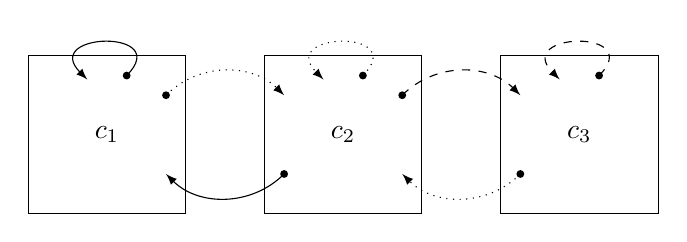
\begin{tikzpicture}
        % Cells
        \draw (0,0) rectangle (2,2) node[midway] {$c_1$};
        \draw (3,0) rectangle (5,2) node[midway] {$c_2$};
        \draw (6,0) rectangle (8,2) node[midway] {$c_3$};

        % Arrows
        \node[circle,fill,inner sep=1pt] at (1.25, 1.75) {};
        \draw[-latex] (1.25, 1.75) to[out=45, in=135, distance=.85cm] (.75, 1.70);

        \node[circle,fill,inner sep=1pt] at (3.25, .5) {};
        \draw[-latex] (3.25, .5) to[out=-135, in=-45] (1.75, .5);


        \node[circle,fill,inner sep=1pt] at (4.25, 1.75) {};
        \draw[-latex, dotted] (4.25, 1.75) to[out=45, in=135, distance=.85cm] (3.75, 1.70);

        \node[circle,fill,inner sep=1pt] at (6.25, .5) {};
        \draw[-latex, dotted] (6.25, .5) to[out=-135, in=-45] (4.75, .5);

        \node[circle,fill,inner sep=1pt] at (1.75, 1.5) {};
        \draw[-latex, dotted] (1.75, 1.5) to[out=45, in=135] (3.25, 1.5);

        
        \node[circle,fill,inner sep=1pt] at (4.75, 1.5) {};
        \draw[-latex, dashed] (4.75, 1.5) to[out=45, in=135] (6.25, 1.5);

        \node[circle,fill,inner sep=1pt] at (7.25, 1.75) {};
        \draw[-latex, dashed] (7.25, 1.75) to[out=45, in=135, distance=.85cm] (6.75, 1.70);
    \end{tikzpicture}
    \caption{Multiple identical reference are needed for a doubly linked list implementation}
    \label{fig:doubly-linked-list-reference}
\end{figure}

This data structure is particularly interesting, as it, unlike the former two presented structures, cannot be expressed in \textsc{Roopl}, as this requires multiple reference to objects, in order for an object to point to itself and to its left and right neighbours. Figure~\ref{fig:doubly-linked-list-reference} shows the multiple references needed for the doubly linked list implementation denoted by the three different arrow types.

\begin{figure}[ht!]
    \centering
    \begin{lstlisting}[style = basic, language = roopl] 
    class DoublyLinkedList
        Cell head
        int length
    
        method appendCell(Cell cell)
            if head = nil & cell != nil then
                head <=> cell
            else skip
            fi head != nil & cell = nil
    
            if head != nil then 
                call head::append(cell)
            else skip
            fi head != nil
    
            length += 1
    \end{lstlisting}
    \caption{Doubly Linked List class}
    \label{fig:doubly-linked-list-class}
\end{figure}

When we append a cell to the list, we first search recursively through the list until we are at the end. The new cell is then set as \textit{right} of the current cell. A reference to the current self is created using the \textbf{copy} statement, and set as \textit{left} of the new end of the list, thus resulting in the new cell being linked to list and now acting as end of the list.

\begin{figure}[ht!]
    \centering
    \begin{lstlisting}[style = basic, language = roopl] 
        class Cell
        int data
        int index
        Cell left
        Cell right
        Cell self
    
        method setData(int value)
            data ^= value
    
        method setIndex(int i)
            index ^= i    
    
        method setLeft(Cell cell)
            left <=> cell
    
        method setRight(Cell cell)
            right <=> cell
    
        method setSelf(Cell cell)
            self <=> cell
    \end{lstlisting}
    \caption{Doubly Linked List Cell class}
    \label{fig:doubly-linked-list-cell-class}
\end{figure}

\begin{figure}[ht!]
    \centering
    \begin{lstlisting}[style = basic, language = roopl]
    method append(Cell cell)
        if right = nil & cell != nil then   // If current cell does not have a right neighbour
            right <=> cell                  // Set new cell as right neighbour of current cell
        
            local Cell selfCopy = nil      
            copy Cell self selfCopy         // Copy reference to current cell
            call right::setLeft(selfCopy)   // Set current as left of  right neighbour
            delocal Cell selfCopy = nil

            local int cellIndex = index + 1
            call right::setIndex(cellIndex) // Set index in right neighbour of current
            delocal int cellIndex = index + 1
        else skip
        fi right != nil & cell = nil

        if right != nil then
            call right::append(cell)        // Keep searching for empty right neighbour
        else skip
        fi right != nil 
    \end{lstlisting}
    \caption{Doubly Linked List Cell class (cont)}
    \label{fig:doubly-linked-list-cell-class-cont}
\end{figure}

The data structure could relatively easily be extended to work as a dynamic array. Currently each cell contains an \textit{index} field, specifying their position in the list. If, say, we wanted to insert some new data at index $n$, without updating the existing value, but essentially squeezing in a new cell, we could add a method to the \textit{DoublyLinkedList} class taking a data value and an index. When executing this method, we could iterate the list until we reach the cell with index $n$, construct a new \textit{cell} instance, update required \textit{left} and \textit{right} pointers to insert the new cell at the correct position, in such a way that the old cell at index $n$ now is the new right neighbour of the cell and finally recursively iterating the list, incrementing the index of cells to the right of the new cell by one. In reverse, this would remove a cell from the list. If we want to update an existing value at a index, a similar technique could be used, where we iterate through the cells until we find the correct index. If we are given an index that is out of bounds in terms of the current length of the list, we could extend the tail on the list until reach a cell with the wanted index. When we are zero-clearing a value that is the furthest index, the inverse would apply, and a such we would zero-clear the cell, and the deallocate cells until we reach a cell which does not have a zero-cleared \textit{data} field. 

This extended doubly linked list would also allow lists of n-dimensional lists, as the type of the \textit{data} field simply could be changed to, say, a \textit{FooDoublyLinkedList}, resulting in an array of Foo arrays. 
\newpage


\section{Type System}
\label{sec:type-system}
The type system of \rooplpp expands on the type system of \textsc{Roopl} presented by~\citeauthor{th:roopl}~\cite{th:roopl} and is analogously described by syntax-directed inference typing rules in the style of ~\citeauthor{wi:semantics}~\cite{wi:semantics}. As \rooplpp introduces two new types in form of \textit{references} and arrays, a few \textsc{Roopl} typing rules must be modified to accommodate these added types. For completeness all typing rules, including unmodified rules, are included in the following sections. 

\subsection{Preliminaries}
\label{subsec:preliminaries}
The types in \rooplpp are given by the following grammar:
\begin{equation*}
    \tau ::= \textbf{int}\ |\ c \in \text{ClassIDs}\ |\ r \in \text{ReferenceIDs}\ |\ i \in \text{IntegerArrayIDs}\ |\ o \in \text{ClassArrayIDs}
\end{equation*}
The type environment $\Pi$ is a finite map pairing variables to types, which can be applied to an identifier $x$ using the $\Pi(x)$ notation. Notation $\Pi' = \Pi[x \mapsto \tau]$ defines updates and creation of a new type environment $\Pi'$ such that $\Pi'(x) = \tau$ and $\Pi'(y) = \Pi(y)$ if $x \not= y$, for some variable identifier $x$ and $y$. The empty type environment is denoted as $[\ ]$ and the function $vars\ :\ Expressions\ \to \text{VarIDs}$ is described by the following definition
\begin{align*}
    &\text{vars}(\bar{n}) &&= \emptyset\\
    &\text{vars}(\textbf{nil}) &&= \emptyset\\
    &\text{vars}(x) &&= \{\ x\ \}\\
    &\text{vars}(x[e]) &&= \{\ x\ \} \cup \text{vars}(e)\\
    &\text{vars}(e_1 \otimes e_2) &&= \text{vars}(e_1) \cup \text{vars}(e_2).
\end{align*}
The binary subtype relation $c_1 \prec: c_2$ is required for supporting subtype polymorphism and is defined as follows:
\begin{align*}
    c_1 &\prec: c_2 &&\text{if}\ c_1\ \text{inherits from}\ c_2\\
    c   &\prec: c   &&(reflexivity)\\
    c_1 &\prec: c_3 &&\text{if}\ c_1 \prec: c_2\ \text{and}\ c_2 \prec: c_3\ (transitivity)
\end{align*}

Furthermore, we formally define object models in such a way that inherited fields and methods are included, unless overridden by the derived fields. Therefore, we define $\Gamma$ to be the class map of a program $p$, such that $\Gamma$ is a finite map from class identifiers to tuples of methods and fields for the class $p$. Application of a class map $\Gamma$ to some class $cl$ is denoted as $\Gamma(cl)$. Construction of a class map is done through function $gen$, as shown in figure~\ref{fig:class-gen}. Figure~\ref{fig:fields-methods} defines the $fields$ and $methods$ functions to determine these given a class. Set operation $\uplus$ defines method overloading by dropping base class methods if a similarly named method exists in the derived class. The definitions shown in Figure~\ref{fig:class-gen} and~\ref{fig:fields-methods} are originally from~\cite{th:roopl}.
 
\begin{figure}[ht]
    \centering
    $\text{gen}\Big(\overbrace{cl_1,\ ...,\ cl_n}^p\Big) = \overbrace{\Big[ \alpha(cl_1) \mapsto \beta(cl_1),\ ...,\ \alpha(cl_n) \mapsto \beta(cl_n) \Big]}^\Gamma$\\

    \vskip 2em
    
    $\alpha\Big(\textbf{class}\ c\ \cdots\Big) = c$
    \hskip 2em
    $\beta(cl) = \Big(\text{fields}(cl),\ \text{methods}(cl) \Big)$

    \caption{Definition $gen$ for constructing the finite class map $\Gamma$ of a given program $p$, originally from ~\cite{th:roopl}}
    \label{fig:class-gen}
\end{figure}

\begin{figure}[H]
    \centering
    \begin{equation*}
        \text{fields}(cl) = \begin{cases}
            \eta(cl)  & \text{if}\ cl \sim [ \textbf{class}\ c\ \cdots ]\\
            \eta(cl) \cup \text{fields}\Big(\alpha^{-1}(c')\Big) & \text{if}\ cl \sim [ \textbf{class}\ c\ \textbf{inherits}\ c'\ \cdots ]
        \end{cases}
    \end{equation*}

    \vskip 1em

    \begin{equation*}
        \text{methods}(cl) = \begin{cases}
            \delta(cl) & \text{if}\ cl \sim [ \textbf{class}\ c\ \cdots ]\\
            \delta(cl) \uplus \text{methods}\Big(\alpha^{-1}(c')\Big) & \text{if}\ cl \sim [\textbf{class}\ c\ \textbf{inherits}\ c'\ \cdots]
        \end{cases}
    \end{equation*}

    \vskip 1em

    \begin{equation*}
        A\ \uplus B\ \overset{def}{=}\ A \cup \bigg\{ m \in B\ \bigg\vert\ \nexists\  m' \Big( \zeta(m') = \zeta(m) \wedge m' \in A \Big) \bigg\}
    \end{equation*}

    $\zeta\Big( \textbf{method}\ q\ (\cdots)\ s \Big) = q$
    \hskip 2em
    $\eta\Big( \textbf{class}\ c\ \cdots\ \overbrace{t_1 f_1\ \cdots\ t_n f_n}^{fs}\ \cdots \Big) = fs$

    \begin{equation*}
        \delta\Big( \textbf{class}\ c\ \cdots \overbrace{\textbf{method}\ q_1\ (\cdots)\ s_1\ \cdots\ \textbf{method}\ q_n\ (\cdots)\ s_n }^{ms}\ \cdots \Big) = ms
    \end{equation*}
    \caption{Definition of fields and methods, originally from~\cite{th:roopl}}
    \label{fig:fields-methods}
\end{figure}

Finally, we formally define a link between arrays of a given type and other types. The function \textit{arrayType}, defined in figure~\ref{fig:array-type}, is $c$ if the passed array $a$ is an array of class $c$ instances.

\begin{figure}[ht]
    \centering
    \begin{equation*}
        \text{arrayType}(a) = \begin{cases}
            c  & \text{if}\ a \in ClassArrayIDs\ \text{and}\ a\ \text{is a}\ c\ \text{array}\\
            \textbf{int} & \text{if}\ a \in i
        \end{cases}
    \end{equation*}
    \caption{Definition \textit{arrayType} for mapping types of arrays to either class types or the integer type}
    \label{fig:array-type}
\end{figure}

\newpage
\subsection{Expressions}
\label{subsec:expressions}
The type judgment

\begin{prooftree}
	\AXC{}
    \UIC{$\Pi \vdash_{expr}\ e : \tau$} 
\end{prooftree} 

defines the type of expressions. The judgment reads as: under type environment $\Pi$, expression $e$ has type $\tau$.

\begin{figure}[ht]
    \begin{center}
        \AXC{} % Con
        \RL{\textsc{T-Con}}
        \UIC{$\Pi \vdash_{expr}\ n : \textbf{int}$} 
        \DP
        \hskip 2em % Var
        \AXC{$\Pi(x) = \tau$}
        \RL{\textsc{T-Var}}
        \UIC{$\Pi \vdash_{expr}\ x : \tau$} 
        \DP
        \hskip 2em % Nil
        \AXC{$\tau \not= \textbf{int}$}
        \RL{\textsc{T-Nil}}
        \UIC{$\Pi \vdash_{expr}\ \textbf{nil}\ : \tau$}
        \DP
        
        \vskip 2em % BinOpInt
        \AXC{$\Pi \vdash_{expr}\ e_1 : \textbf{int}$}
        \AXC{$\Pi \vdash_{expr}\ e_2 : \textbf{int}$}
        \RL{\textsc{T-BinOpInt}}
        \BIC{$\Pi \vdash_{expr}\ e_1 \otimes e_2 : \textbf{int}$}
        \DP

        \vskip 2em % BinOpObj
        \AXC{$\Pi \vdash_{expr}\ e_1 : c$}
        \AXC{$\Pi \vdash_{expr}\ e_2 : c$}
        \AXC{$\otimes \in \{ \texttt{\textbf{=}}, \texttt{\textbf{!=}} \}$}
        \RL{\textsc{T-BinOpObj}}
        \TIC{$\Pi \vdash_{expr}\ e_1 \otimes e_2 : \textbf{int}$}
        \DP
    \end{center}
    \caption{Typing rules for expressions in \textsc{Roopl}, originally from~\cite{th:roopl}}
    \label{fig:typing-rules-expressions}
\end{figure}

The original expression typing rules from \textsc{Roopl} are shown in figure~\ref{fig:typing-rules-expressions}. The type rules \textsc{T-Con}, \textsc{T-Var} and \textsc{T-Nil} defines typing of the simplest expressions. Numeric literals are of type \textbf{int}, typing of variable expressions depends on the type of the variable in the type environment and the \textbf{nil} literal is a non-integer type. All binary operations are defined for integers, while only equality-operators are defined for objects.

With the addition of the \rooplpp array type, we extend the expression typing rules with rule \textsc{T-ArrElemVar} which defines typing for array element variables, shown in figure~\ref{fig:typing-rules-expression-extension}.

\begin{figure}[ht]
    \begin{center}
        \AXC{$\text{arrayType}(x) = \tau$}
        \AXC{$\Pi_{expr} \vdash\ e\ :\ \textbf{int}$}
        % \AXC{$\Pi(x[e]) = \tau$}
        \RL{\textsc{T-ArrElemVar}}
        \BIC{$\Pi \vdash_{expr}\ x[e] : \tau$} 
        \DP
    \end{center}
    \caption{Typing rule extension for the \textsc{Roopl} typing rules}
    \label{fig:typing-rules-expression-extension}
\end{figure}  
 

\subsection{Statements}
\label{subsec:statements}
The type judgment

\begin{prooftree}
	\AXC{}
    \UIC{$\langle \Pi,\ c\rangle\ \vdash_{stmt}^\Gamma\ s$} 
\end{prooftree} 

defines well-typed statements. The judgment reads as under type environment $\Pi$ within class $c$, statement $s$ is well-typed with class map $\Gamma$.
\begin{figure}[H]
    \begin{center}
        % Assignment
        \AXC{$x \not\in \text{vars}(e)$}
        \AXC{$\Pi \vdash_{expr}\ e : \textbf{int}$}
        \AXC{$\Pi(x) = \textbf{int}$}
        \RL{\textsc{T-AssVar}}
        \TIC{$\langle \Pi, c \rangle \vdash^{\Gamma}_{stmt}\ x\ \texttt{$\odot$=}\ e$}
        \DP

        \vskip 2em
        
        % If
        \AXC{$\Pi \vdash_{expr}\ e_1 : \textbf{int}$}
        \AXC{$\langle \Pi, c \rangle \vdash^{\Gamma}_{stmt}\ s_1$}
        \AXC{$\langle \Pi, c \rangle \vdash^{\Gamma}_{stmt}\ s_2$}
        \AXC{$\Pi \vdash_{expr}\ e_2 : \textbf{int}$}
        \RL{\textsc{T-If}}
        \QIC{$\langle \Pi, c \rangle \vdash^{\Gamma}_{stmt}\ \textbf{if}\ e_1\ \textbf{then}\ s_1\ \textbf{else}\ s_2\ \textbf{fi}\ e_2$}
        \DP

        \vskip 2em

        % Loop
        \AXC{$\Pi \vdash_{expr}\ e_1 : \textbf{int}$}
        \AXC{$\langle \Pi, c \rangle \vdash^{\Gamma}_{stmt}\ s_1$}
        \AXC{$\langle \Pi, c \rangle \vdash^{\Gamma}_{stmt}\ s_2$}
        \AXC{$\Pi \vdash_{expr}\ e_2 : \textbf{int}$}
        \RL{\textsc{T-Loop}}
        \QIC{$\langle \Pi, c \rangle \vdash^{\Gamma}_{stmt}\ \textbf{from}\ e_1\ \textbf{do}\ s_1\ \textbf{loop}\ s_2\ \textbf{until}\ e_2$}
        \DP

        \vskip 2em
        
        % ObjectBlock + Skip
        \AXC{$\langle \Pi[x \mapsto c'], c \rangle \vdash^{\Gamma}_{stmt}\ s$}
        \RL{\textsc{T-ObjBlock}}
        \UIC{$\langle \Pi, c \rangle \vdash^{\Gamma}_{stmt}\ \textbf{construct}\ c'\ x\quad s\quad \textbf{destruct}\ x$} 
        \DP
        \hskip 2em
        \AXC{}
        \RL{\textsc{T-Skip}}
        \UIC{$\langle \Pi, c \rangle \vdash^{\Gamma}_{stmt}\ \textbf{skip}$} 
        \DP

        \vskip 2em

        % Seq + SwapVar
        \AXC{$\langle \Pi, c \rangle \vdash^{\Gamma}_{stmt}\ s_1$}
        \AXC{$\langle \Pi, c \rangle \vdash^{\Gamma}_{stmt}\ s_2$}
        \RL{\textsc{T-Seq}}
        \BIC{$\langle \Pi, c \rangle \vdash^{\Gamma}_{stmt}\ s_1\ s_2$}
        \DP
        \hskip 2em
        \AXC{$\Pi(x_1) = \Pi(x_2)$}
        \RL{\textsc{T-SwpVar}}
        \UIC{$\langle \Pi, c \rangle \vdash^{\Gamma}_{stmt}\ x_1\ \texttt{\textbf{<=>}}\ x_2$}
        \DP

        \vskip 2em

        % T-Call
        \AXC{$\Gamma(\Pi(c)) = \Big( fields,\ methods \Big)$}
        \DP
        \AXC{$\Big( \textbf{method}\ q(t_1\ y_1,\ ...,\ t_n\ y_n)\ s \Big) \in methods$}
        \DP
        \AXC{$\{ x_1,\ ...,\ x_n \} \cap fields = \emptyset$}
        \AXC{$i \not= j \implies x_i \not= x_j$}
        \AXC{$\Pi(x_1) \prec: t_1\ \cdots\ \Pi(x_n) \prec: t_n$}
        \RL{\textsc{T-Call}}
        \TIC{$\langle \Pi, c \rangle \vdash^{\Gamma}_{stmt}\ \textbf{call}\ q(x_1,\ ...,\ x_n)$}
        \DP

        \vskip 2em
        
        % T-CallO
        \AXC{$\Gamma(\Pi(x_0)) = \Big( fields,\ methods \Big)$}
        \DP
        \AXC{$\Big( \textbf{method}\ q(t_1\ y_1,\ ...,\ t_n\ y_n)\ s \Big) \in methods$}
        \DP
        \AXC{$i \not= j \implies x_i \not= x_j$}
        \AXC{$\Pi(x_1) \prec: t_1\ \cdots\ \Pi(x_n) \prec: t_n$}
        \RL{\textsc{T-CallO}}
        \BIC{$\langle \Pi, c \rangle \vdash^{\Gamma}_{stmt}\ \textbf{call}\ x_0::q(x_1,\ ...,\ x_n)$}
        \DP

        \vskip 2em

        % UC and UCO
        \AXC{$\langle \Pi, c \rangle \vdash^{\Gamma}_{stmt}\ \textbf{call}\ q(x_1,\ ...,\ x_n)$}
        \RL{\textsc{T-Uc}}
        \UIC{$\langle \Pi, c \rangle \vdash^{\Gamma}_{stmt}\ \textbf{uncall}\ q(x_1,\ ...,\ x_n)$}
        \DP
        \hskip 2em
        \AXC{$\langle \Pi, c \rangle \vdash^{\Gamma}_{stmt}\ \textbf{call}\ x_0::q(x_1,\ ...,\ x_n)$}
        \RL{\textsc{T-Uco}}
        \UIC{$\langle \Pi, c \rangle \vdash^{\Gamma}_{stmt}\ \textbf{uncall}\ x_0::q(x_1,\ ...,\ x_n)$}
        \DP
    \end{center}
    \caption{Typing rules for statements in \textsc{Roopl}, originally from~\cite{th:roopl}}
    \label{fig:typing-rules-statements}
\end{figure}

Typing rule \textsc{T-AssVar} defines variable assignments for an integer variable and an integer expression result, given that the variable $x$ does not occur in the expression $e$. 

The type rules \textsc{T-If} and \textsc{T-Loop} defines reversible conditionals and loops as known from \textsc{Janus}, where entry and exit conditions are integers and branch and loop statements are well-typed statements. 

The object block, introduced in \textsc{Roopl}, is only well-typed if its body statement is well-typed. 

The \textbf{skip} statement is always well-typed, while a sequence of statements are well-typed if each of the provided statements are. Variable \textbf{swap} statements are well-typed if both operands are of the same type under type environment $\Pi$.

As with \textsc{Roopl}, type correctness of local method invocation is defined in rule \textsc{T-Call} iff:
\begin{itemize}
    \item The number of arguments matches the method arity
    \item No class fields are present in the arguments passed to the method (To prevent irreversible updates)
    \item The argument list contains unique elements
    \item Each argument is a subtype of the type of the equivalent formal parameter. 
\end{itemize}

For foreign method invocations, typing rule \textsc{T-CallO}. A foreign method invocation is well-typed using the same rules as for \textsc{T-Call} besides having no restrictions on class fields parameters in the arguments, but an added rule stating that the callee object $x_0$ must not be passed as an argument.

The typing rules \textsc{T-UC} and \textsc{T-UCO} defines uncalling of methods in terms of their respective inverse counterparts.

\begin{figure}[H]
    \begin{center}
        % Assignment
        \AXC{$\Pi(x) = \textbf{int}[\ ]$}
        \DP
        \AXC{$\Pi \vdash_{expr} e_1\ :\ \textbf{int}$}
        \DP
        \vskip 1em
        \AXC{$x \not\in \text{vars}(e_2)$}
        \AXC{$\text{vars}(e_1) \wedge \text{vars}(e_2) = \emptyset$}
        \AXC{$\Pi \vdash_{expr}\ e_2 : \textbf{int}$}
        \RL{\textsc{T-ArrElemAss}}
        \TIC{$\langle \Pi, c \rangle \vdash^{\Gamma}_{stmt}\ x[e_1] \odot= e_2$}
        \DP 

        \vskip 2em
         % Object new + delete
        \AXC{$\Pi(x) = c'$}
        \RL{\textsc{T-ObjNew}}
        \UIC{$\langle \Pi, c \rangle  \vdash^{\Gamma}_{stmt}\ \textbf{new}\ c'\ x$} 
        \DP
        \hskip 2em
        \AXC{$\Pi(x) = c'$}
        \RL{\textsc{T-ObjDlt}}
        \UIC{$\langle \Pi, c \rangle  \vdash^{\Gamma}_{stmt}\ \textbf{delete}\ c'\ x$} 
        \DP

        \vskip 2em

         % Array new
         \AXC{$\text{arrayType}(a) \in \Big\{ \text{classIDs}, \textbf{int} \Big\}$}
         \AXC{$\Pi \vdash_{expr}\ e = \textbf{int}$}
         \AXC{$\Pi(x) = a[\ ]$}
         \RL{\textsc{T-ArrNew}}
         \TIC{$\langle \Pi, c \rangle  \vdash^{\Gamma}_{stmt}\ \textbf{new}\ a[e]\ x$} 
         \DP

         \vskip 2em

         % Array delete
         \AXC{$\text{arrayType}(a) \in \Big\{ \text{classIDs}, \textbf{int} \Big\}$}
         \AXC{$\Pi \vdash_{expr}\ e = \textbf{int}$}
         \AXC{$\Pi(x) = a[\ ]$}
         \RL{\textsc{T-ArrDlt}}
         \TIC{$\langle \Pi, c \rangle  \vdash^{\Gamma}_{stmt}\ \textbf{delete}\ a[e]\ x$}
         \DP
 
         \vskip 2em

        % Copy + uncopy
        \AXC{$\Pi(x) = c'$}
        \AXC{$\Pi(x') = c'$}
        \RL{\textsc{T-Cp}}
        \BIC{$\langle \Pi, c \rangle  \vdash^{\Gamma}_{stmt}\ \textbf{copy}\ c'\ x\ x'$} 
        \DP
        \hskip 2em
        \AXC{$\Pi(x) = c'$}
        \AXC{$\Pi(x') = c'$}
        \RL{\textsc{T-Ucp}}
        \BIC{$\langle \Pi, c \rangle  \vdash^{\Gamma}_{stmt}\ \textbf{uncopy}\ c'\ x\ x'$}
        \DP

        \vskip 2em

        % Local block
        \AXC{$\langle \Pi, c \rangle \vdash_{expr}\ e_1\ :\ c'$}
        \AXC{$\langle \Pi[x \mapsto c'], c \rangle \vdash^{\Gamma}_{stmt}\ s$}
        \AXC{$\langle \Pi, c \rangle \vdash_{expr}\ e_2\ :\ c'$}
        \RL{\textsc{T-LocalBlock}}
        \TIC{$\langle \Pi, c \rangle \vdash^{\Gamma}_{stmt}\ \textbf{local}\ c'\ x = e_1\quad s\quad \textbf{delocal}\ c'\ x = e_2$} 
        \DP
    \end{center}
    \caption{Typing rules extensions for statements in \rooplpp}
    \label{fig:typing-rules-statements-extensions}
\end{figure}

Figure~\ref{fig:typing-rules-statements-extensions} shows the typing rules for the extensions made to \textsc{Roopl} in \rooplpp, covering the \textbf{new}/\textbf{delete} and \textbf{copy}/\textbf{uncopy} statements for objects and arrays and local blocks.

The typing rule \textsc{T-ArrElemAss} defines assignment to integer array element variables, and is well-typed when the type of array $x$ is \textbf{int}, the variable $x[e_1]$ is not present in the right-hand side of the statement and both expressions $e_1$ and $e_2$ evaluates to integers.

The \textsc{T-ObjNew} and \textsc{T-ObjDlt} rules define well-typed \textbf{new} and \textbf{delete} statements for dynamically lifetimed objects. The \textbf{new} statement is well-typed, as long as $c' \in \text{classIDs}$ and the variable $x$ is a \textbf{nil}-type and the \textbf{delete} is well-typed if the type of $x$ under type environment $\Pi$ is equal to $c'$.

The \textsc{T-ArrNew} and \textsc{T-ArrDlt} rules define well-type \textbf{new} and \textbf{delete} statement for \rooplpp arrays. The \textbf{new} statement is well-typed, if the type of the array either is a classID or \textbf{int}, the length expression evaluates to an integer and $x$ is zero-cleared, and \textbf{delete} is well-typed if the type of the array is either a classID or \textbf{int}, the length expression evaluates to an integer and $x$ is equal to the array type $a$.

Typing rules \textsc{T-Cp} and \textsc{T-Ucp} define well-typed reference copy and un-copying statements. A well-typed \textbf{copy} statement requires that the type of $x$ is $c'$ under type environment $\Pi$, while a well-typed \textbf{uncopy} statement further requires that the type of $x'$ is $c'$ too.

The rule \textsc{T-LocalBlock} defines well-typed local blocks. A local block is well-typed if its two expression $e_1$ and $e_2$ are well-typed and its body statement $s$ is well-typed. 

\subsection{Programs}
\label{subsec:programs} 
As with \textsc{Roopl}, a \rooplpp program is well-typed if all of its classes and their respective methods are well-typed and if there exists a nullary main method. Figure~\ref{fig:typing-programs} shows the typing rules for class methods, classes and programs.

\begin{figure}[H]
    \begin{center}
        % Method
        \AXC{$\langle \Pi[x_1 \mapsto t_1,\ ...,\ x_n \mapsto t_n],\ c \rangle \vdash^{\Gamma}_{stmt}\ s$}
        \RL{\textsc{T-Method}}
        \UIC{$\langle \Pi, c \rangle \vdash^{\Gamma}_{meth}\ \textbf{method}\ q(t_1 x_1,\ ...,\ t_n x_n)\ s$}
        \DP

        \vskip 2em

        % Class
        \AXC{$\Gamma(c) = \Big( \overbrace{\big\{ \langle t_1, f_1 \rangle,\ ...,\ \langle t_i, f_i \rangle \big\}}^{fields},\ \overbrace{\{ m_1,\ ...,\ m_n \}}^{methods} \Big)$}
        \DP
        \AXC{$\Pi = \big[ f_1 \mapsto t_1,\ ...,\ f_n \mapsto t_n \big]$}
        \AXC{$\langle \Pi, c \rangle \vdash^{\Gamma}_{meth}\ m_1 \quad \cdots \quad \langle \Pi, c \rangle \vdash^{\Gamma}_{meth}\ m_n$}
        \RL{\textsc{T-Class}}
        \BIC{$\vdash^{\Gamma}_{class}\ c$}
        \DP

        \vskip 2em

        \AXC{$\Big( \textbf{method main ()}\ s \Big) \in \displaystyle\bigcup^{n}_{i = 1} \text{methods}(c_i)$}
        \DP
        \AXC{$\Gamma = \text{gen}(c_1,\ ...,\ c_n)$}
        \AXC{$\vdash^{\Gamma}_{class}\ c_1 \quad \cdots \quad \vdash^{\Gamma}_{class}\ c_n$}
        \RL{\textsc{T-Prog}}
        \BIC{$\vdash_{prog}\ c_1\ \cdots\ c_n$}
        \DP
    \end{center}
    \caption{Typing rules for class methods, classes and programs, originally from~\cite{th:roopl}}
    \label{fig:typing-programs}
\end{figure}

\newpage
\section{Language Semantics}
\label{sec:language-semantics}
The following sections contain the operational semantics of \rooplpp, as specified by syntax-directed inference rules.

\subsection{Preliminaries}
\label{subsec:semantics-preliminaries}
We define a memory location $l$ to be a single location in program memory, where a memory location is in the set of non-negative integers, $\mathbb{N}_0$. An environment $\gamma$ is a partial function mapping variables to memory locations. A store $\mu$ is a partial function mapping memory locations to values. An object is a tuple of a class name and an environment mapping fields to memory locations. A value is either an integer, an object or a memory location.

Applications of environments $\gamma$ and stores $\mu$ are analogous to the type environment $\Gamma$, defined in section~\ref{subsec:preliminaries}. 

\begin{figure}[ht]
    \begin{alignat*}{2}
        l      \in\ &\text{Locs}     &&= \mathbb{N}_0\\
        \gamma \in\ &\text{Envs}     &&= \text{VarIDs} \rightharpoonup \text{Locs}\\
        \mu    \in\ &\text{Stores}   &&= \text{Locs} \rightharpoonup \text{Values}\\
        &\text{Objects} &&= \Big\{ \langle c_f,\ \gamma_f \rangle \mid c_f \in \text{ClassIDs}\ \wedge\ \gamma_f \in \text{Envs} \Big\}\\
        v \in\ &\text{Values} &&= \mathbb{Z} \cup \text{Objects}\ \cup \text{Locs}
    \end{alignat*}
    \caption{Semantic values, originally from~\cite{th:roopl}}
    \label{fig:semantic-values}
\end{figure}

\subsection{Expressions}
\label{subsec:semantics-expressions}
The judgment:
\begin{prooftree}
    \AXC{$\langle \gamma, \mu \rangle \vdash_{expr}\ e \Rightarrow v$}
\end{prooftree}
defines the meaning of expressions. We say that under environment $\gamma$ and store $\mu$, expression $e$ evaluates to value $v$.

\begin{figure}[ht]
    \begin{center}
        \AXC{}
        \RL{\textsc{Con}}
        \UIC{$\langle \gamma, \mu \rangle \vdash_{expr}\ n \Rightarrow \bar{n}$}
        \DP
        \hskip 1.5em
        \AXC{}
        \RL{\textsc{Var}}
        \UIC{$\langle \gamma, \mu \rangle \vdash_{expr}\ x \Rightarrow \mu\Big( \gamma(x) \Big)$}
        \DP
        \hskip 1.5em
        \AXC{}
        \RL{\textsc{Nil}}
        \UIC{$\langle \gamma, \mu \rangle \vdash_{expr}\ \texttt{\textbf{nil}} \Rightarrow 0$}
        \DP

        \vskip 1.5em

        \AXC{$\langle \gamma, \mu \rangle \vdash_{expr}\ e_1 \Rightarrow v_1 $}
        \AXC{$\langle \gamma, \mu \rangle \vdash_{expr}\ e_2 \Rightarrow v_2 $}
        \AXC{$\llbracket \otimes \rrbracket(v_1, v_2) = v$}
        \RL{\textsc{BinOp}}
        \TIC{$\langle \gamma, \mu \rangle \vdash_{expr}\ e_1 \otimes e_2 \Rightarrow v$}
        \DP 
    \end{center}
    \caption{Semantic inference rules for expressions, originally from~\cite{th:roopl}}
    \label{fig:semantics-expr-rules}
\end{figure}

As shown in figure~\ref{fig:semantics-expr-rules}, expression evaluation has no effects on the store. Logical values are represented by \textit{truthy} and \textit{falsy} values of any non-zero value and zero respectively. The evaluation of binary operators is presented in figure~\ref{fig:binary-operator-evaluation}.

\begin{figure}[ht]
    \begin{center}
        \AXC{$\langle \gamma, \mu \rangle \vdash_{expr}\ e \Rightarrow v $}
        \RL{\textsc{ArrElemVar}}
        \UIC{$\langle \gamma, \mu \rangle \vdash_{expr}\ x[e] \Rightarrow \mu\Big( \gamma(x[v]) \Big)$}
        \DP
    \end{center}
    \caption{Extension to the semantic inference rules for expression in \rooplpp}
    \label{sec:semantics-expr-rule-extensions}
\end{figure}

For \rooplpp, we extend the expression ruleset with a single rule for array element variables shown in figure~\ref{sec:semantics-expr-rule-extensions}. As with the expressions inference rules in \textsc{Roopl}, this extension has no effect on the store. 

\begin{figure}[ht]
    \begin{align*}
        &\llbracket \texttt{\textbf{+}} \rrbracket (v_1, v_2) &&= v_1 + v_2 &\llbracket \texttt{\textbf{\%}} \rrbracket (v_1, v_2)      &&&= v_1\ \text{mod}\ v_2\\
        &\llbracket \texttt{\textbf{-}} \rrbracket (v_1, v_2) &&= v_1 - v_2 &\llbracket \texttt{\textbf{\&}} \rrbracket (v_1, v_2)       &&&= v_1 \wedge v_2\\
        &\llbracket \texttt{\textbf{*}} \rrbracket (v_1, v_2) &&= v_1 \times v_2 &\llbracket \texttt{\textbf{|}} \rrbracket  (v_1, v_2) &&&= v_1 \vee v_2\\
        &\llbracket \texttt{\textbf{/}} \rrbracket (v_1, v_2) &&= v_1 \div v_2 &\llbracket \texttt{\textbf{\^}} \rrbracket (v_1, v_2)   &&&= v_1 \oplus v_2\\ 
        &\llbracket\texttt{\textbf{\&\&}}\rrbracket (v_1, v_2) &&= \begin{cases} 
            0 & \text{if}\ v_1 = 0 \vee v_2 = 0\\ 
            1 & \text{otherwise}
        \end{cases}        
        &\llbracket\texttt{\textbf{<=}}\rrbracket (v_1, v_2) &&&= \begin{cases} 
            0 & \text{if}\ v_1 \leq v_2\\ 
            1 & \text{otherwise} 
        \end{cases}\\
        &\llbracket\texttt{\textbf{||}}\rrbracket (v_1, v_2) &&= \begin{cases}
            0 & \text{if}\ v_1 = v_2 = 0\\ 
            1 & \text{otherwise}
        \end{cases}
        &\llbracket\texttt{\textbf{>=}}\rrbracket (v_1, v_2) &&&= \begin{cases}
            0 & \text{if}\ v_1 \geq v_2\\
            1 & \text{otherwise}
        \end{cases}\\
        &\llbracket\texttt{\textbf{<}}\rrbracket (v_1, v_2) &&= \begin{cases}
            0 & \text{if}\ v_1 < v_2\\ 
            1 & \text{otherwise}
        \end{cases}
        &\llbracket\texttt{\textbf{=}}\rrbracket (v_1, v_2) &&&= \begin{cases}
            0 & \text{if}\ v_1 = v_2\\
            1 & \text{otherwise}
        \end{cases}\\
        &\llbracket\texttt{\textbf{>}}\rrbracket (v_1, v_2) &&= \begin{cases}
            0 & \text{if}\ v_1 > v_2\\ 
            1 & \text{otherwise}
        \end{cases}
        &\llbracket\texttt{\textbf{!=}}\rrbracket (v_1, v_2) &&&= \begin{cases}
            0 & \text{if}\ v_1 \not= v_2\\
            1 & \text{otherwise}
        \end{cases}
    \end{align*} 
    \caption{Definition of binary expression operator evaluation, originally from~\cite{th:roopl}}
    \label{fig:binary-operator-evaluation}
\end{figure}


\subsection{Statements}
\label{subsec:semantics-statements}
The judgment
\begin{prooftree}
    \AXC{$\langle l, \gamma \rangle \vdash^{\Gamma}_{stmt}\ s : \mu \rightleftharpoons \mu'$}
\end{prooftree}
defines the meaning of statements. We say that under environment $\gamma$ and object $l$, statement $s$ with class map $\Gamma$ reversibly transforms store $\mu$ to store $\mu'$, where $l$ is the location of the current object in the store. Figure~\ref{fig:semantic-statements},~\ref{fig:semantic-statements-cont} and~\ref{fig:semantic-statements-cont2} defines the operational semantics of \rooplpp.

\begin{subfigures}
    \begin{figure}[!ht]
        \begin{center}
            % Skip
            \AXC{}
            \RL{\textsc{Skip}}
            \UIC{$\langle l, \gamma \rangle \vdash^{\Gamma}_{stmt}\ \textbf{skip} : \mu \rightleftharpoons \mu$}
            \DP
    
            \vskip 2em
    
            % Seq
            \AXC{$\langle l, \gamma \rangle \vdash^{\Gamma}_{stmt}\ s_1 : \mu \rightleftharpoons \mu'$}
            \AXC{$\langle l, \gamma \rangle \vdash^{\Gamma}_{stmt}\ s_2 : \mu' \rightleftharpoons \mu''$}
            \RL{\textsc{Seq}}
            \BIC{$\langle l, \gamma \rangle \vdash^{\Gamma}_{stmt}\ s_1\ s_2 : \mu \rightleftharpoons \mu''$}
            \DP
    
            \vskip 2em
    
            % AssVar
            \AXC{$\langle \gamma, \mu \rangle \vdash^{\Gamma}_{stmt}\ e \Rightarrow v$}
            \AXC{$\llbracket \odot \rrbracket \Big( \mu \Big( \gamma(x) \Big), v \Big) = v'$}
            \RL{\textsc{AssVar}}
            \BIC{$\langle l, \gamma \rangle \vdash^{\Gamma}_{stmt}\ x \odot= e\ :\ \mu \rightleftharpoons \mu[\gamma(x) \mapsto v']$}
            \DP
    
            \vskip 2em
    
            % SwpVar
            \AXC{$\mu \Big( \gamma(x_1) \Big) = v_1$}
            \AXC{$\mu \Big( \gamma(x_2) \Big) = v_2$}
            \RL{\textsc{SwpVar}}
            \BIC{$\langle l, \gamma \rangle \vdash^{\Gamma}_{stmt}\ x_1\ \texttt{\textbf{<=>}}\ x_2\ :\ \mu \rightleftharpoons \mu[\gamma(x_1) \mapsto v_2,\ \gamma(x_2) \mapsto v_1]$}
            \DP
    
            \vskip 2em
    
            % Loop Main
            \AXC{$\langle \gamma, \mu \rangle \vdash^{\Gamma}_{expr}\ e_1 \not\Rightarrow 0$}
            \AXC{$\langle l, \gamma \rangle \vdash^{\Gamma}_{stmt}\ s_1 : \mu \rightleftharpoons \mu'$}
            \AXC{$\langle l, \gamma \rangle \vdash^{\Gamma}_{loop}\ (e_1, s_1, s_2, e_2) : \mu' \rightleftharpoons \mu''$}
            \RL{\textsc{LoopMain}}
            \TIC{$\langle l, \gamma \rangle \vdash^{\Gamma}_{stmt}\ \textbf{from}\ e_1\ \textbf{do}\ s_1\ \textbf{loop}\ s_2\ \textbf{until}\ e_2\ :\ \mu \rightleftharpoons \mu''$}
            \DP
    
            \vskip 2em
    
            % Loop Base
            \AXC{$\langle \gamma, \mu \rangle \vdash^{\Gamma}_{expr}\ e_2 \not\Rightarrow 0$}
            \RL{\textsc{LoopBase}}
            \UIC{$\langle l, \gamma \rangle \vdash^{\Gamma}_{loop}\ (e_1, s_1, s_2, e_2)\ :\ \mu \rightleftharpoons \mu$}
            \DP
    
            \vskip 2em
    
            % Loop Rec
            \AXC{$\langle \gamma, \mu \rangle \vdash^{\Gamma}_{expr} e_2 \Rightarrow 0$}
            \DP
            \hskip 8em
            \AXC{$\langle l, \gamma \rangle \vdash^{\Gamma}_{stmt} s_2 : \mu \rightleftharpoons \mu'$}
            \DP
            \vskip 0.5em
            \AXC{$\langle \gamma, \mu' \rangle \vdash^{\Gamma}_{expr} e_1 \Rightarrow 0$}
            \AXC{$\langle l, \gamma \rangle \vdash^{\Gamma}_{stmt} s_1 : \mu' \rightleftharpoons \mu''$}
            \AXC{$\langle l, \gamma \rangle \vdash^{\Gamma}_{loop} (e_1, s_1, s_2, e_2) : \mu'' \rightleftharpoons \mu'''$}
            \RL{\textsc{LoopRec}}
            \TIC{$\langle l, \gamma \rangle \vdash^{\Gamma}_{loop}\ (e_1, s_1, s_2, e_2)\ :\ \mu \rightleftharpoons \mu'''$}
            \DP
    
            \vskip 2em
    
            % If True
            \AXC{$\langle \gamma, \mu \rangle \vdash^{\Gamma}_{expr} e_1 \not\Rightarrow 0$}
            \AXC{$\langle l, \gamma \rangle \vdash^{\Gamma}_{stmt} s_1 : \mu \rightleftharpoons \mu'$}
            \AXC{$\langle \gamma, \mu' \rangle \vdash^{\Gamma}_{expr} e_2 \not\Rightarrow 0$}
            \RL{\textsc{IfTrue}}
            \TIC{$\langle l, \gamma \rangle \vdash^{\Gamma}_{stmt}\ \textbf{if}\ e_1\ \textbf{then}\ s_1\ \textbf{else}\ s_2\ \textbf{fi}\ e_2\ :\ \mu \rightleftharpoons \mu'$}
            \DP
    
            \vskip 2em
    
            % If False
            \AXC{$\langle \gamma, \mu \rangle \vdash^{\Gamma}_{expr} e_1 \Rightarrow 0$}
            \AXC{$\langle l, \gamma \rangle \vdash^{\Gamma}_{stmt} s_1 : \mu \rightleftharpoons \mu'$}
            \AXC{$\langle \gamma, \mu' \rangle \vdash^{\Gamma}_{expr} e_2 \Rightarrow 0$}
            \RL{\textsc{IfFalse}}
            \TIC{$\langle l, \gamma \rangle \vdash^{\Gamma}_{stmt}\ \textbf{if}\ e_1\ \textbf{then}\ s_1\ \textbf{else}\ s_2\ \textbf{fi}\ e_2\ :\ \mu \rightleftharpoons \mu'$}
            \DP
        \end{center}
        \caption{Semantic inference rules for statements, originally from~\cite{th:roopl}}
        \label{fig:semantic-statements}
    \end{figure}
    
    \begin{figure}[!ht]
        \begin{center}           
            % Call
            \AXC{$\mu(l) = \langle c, \gamma' \rangle $}
            \DP
            \AXC{$\Gamma(c) = (fields, methods)$}
            \DP
            \AXC{$\Big( \textbf{method}\ q(t_1 y_1,\ ...,\ t_n y_n)\ s \Big) \in methods$}
            \DP
            \AXC{$\Big\langle l, \gamma'[y_1 \mapsto \gamma(x_1),\ ...,\ y_n \mapsto \gamma(x_n)] \Big\rangle \vdash^{\Gamma}_{stmt}\ s : \mu \rightleftharpoons \mu'$}
            \RL{\textsc{Call}}
            \UIC{$\langle l, \gamma \rangle \vdash^{\Gamma}_{stmt}\ \textbf{call}\ q(x_1,\ ...,\ x_n)\ :\ \mu \rightleftharpoons \mu'$}
            \DP
    
            \vskip 2em
    
            % Uncall
            \AXC{$\langle l, \gamma \rangle \vdash^{\Gamma}_{stmt}\ \textbf{call}\ q(x_1,\ ...,\ x_n)\ :\ \mu' \rightleftharpoons \mu$}
            \RL{\textsc{Uncall}}
            \UIC{$\langle l, \gamma \rangle \vdash^{\Gamma}_{stmt}\ \textbf{uncall}\ q(x_1,\ ...,\ x_n)\ :\ \mu \rightleftharpoons \mu'$}
            \DP

            \vskip 2em

            % Object call
            \AXC{$l' = \mu\Big( \gamma(x_0) \Big) $}
            \DP
            \AXC{$\mu(l') = \langle c, \gamma' \rangle $}
            \DP
            \AXC{$\Gamma(c) = (fields, methods)$}
            \DP
            \AXC{$\Big( \textbf{method}\ q(t_1 y_1,\ ...,\ t_n y_n)\ s \Big) \in methods$}
            \DP
            \AXC{$\Big\langle l', \gamma'[y_1 \mapsto \gamma(x_1),\ ...,\ y_n \mapsto \gamma(x_n)] \Big\rangle \vdash^{\Gamma}_{stmt}\ s : \mu \rightleftharpoons \mu'$}
            \RL{\textsc{CallObj}}
            \UIC{$\langle l, \gamma \rangle \vdash^{\Gamma}_{stmt}\ \textbf{call}\ x_0::q(x_1,\ ...,\ x_n)\ :\ \mu \rightleftharpoons \mu'$}
            \DP
    
            \vskip 2em
            
            % Object Uncall
            \AXC{$\langle l, \gamma \rangle \vdash^{\Gamma}_{stmt}\ \textbf{call}\ x_0::q(x_1,\ ...,\ x_n)\ :\ \mu' \rightleftharpoons \mu$}
            \RL{\textsc{ObjUncall}}
            \UIC{$\langle l, \gamma \rangle \vdash^{\Gamma}_{stmt}\ \textbf{uncall}\ x_0::q(x_1,\ ...,\ x_n)\ :\ \mu \rightleftharpoons \mu'$}
            \DP
        \end{center}
        \caption{Semantic inference rules for statements, originally from~\cite{th:roopl} (cont)}
        \label{fig:semantic-statements-cont}
    \end{figure}

    \begin{figure}[!ht]
        \begin{center}
            % Object block
            \AXC{$\Gamma(c) = \Big( \overbrace{\{\langle t_1, f_1 \rangle,\ ...,\ \langle t_n, f_n \rangle \}}^{fields}, methods \Big)$}
            \DP
            \AXC{$\gamma' = [f_1 \mapsto a_1,\ ...,\ f_n \mapsto a_n]$}
            \DP
            \vskip 1em
            \AXC{$\{ l', r, a_1, ..., a_n \} \cap \text{dom}(\mu) = \emptyset$}
            \DP
            \AXC{$|\{ l', r, a_1, ..., a_n \}| = n + 2$}
            \DP
            \vskip 1em
            \AXC{$\mu' = \mu\Big[ a_1 \mapsto 0,\ ...,\ a_n \mapsto 0,\ l' \mapsto \langle c, \gamma' \rangle,\ r \mapsto l' \Big]$}
            \DP
            \vskip 1em
            \AXC{$\langle l, \gamma[x \mapsto r] \rangle \vdash^{\Gamma}_{stmt}\ s : \mu' \rightleftharpoons \mu''$}
            \AXC{$\mu''(a_1) = 0\ \cdots\ \mu''(a_n) = 0$}
            \RL{\textsc{ObjBlock}}
            \BIC{$\langle l, \gamma \rangle \vdash^{\Gamma}_{stmt}\ \textbf{construct}\ c\ x \quad s \quad \textbf{destruct}\ x\ :\ \mu \rightleftharpoons \mu'' \upharpoonright_{\text{dom}(\mu)}$}  
            \DP
        \end{center}
        \caption{Semantic inference rules for statements, originally from~\cite{th:roopl} (cont)}
        \label{fig:semantic-statements-cont2}
    \end{figure}

    \begin{figure}[!ht]
        \begin{center}   
            % AssArrElemVar
            \AXC{$\langle \gamma, \mu \rangle \vdash^{\Gamma}_{stmt}\ e_1 \Rightarrow v_1$}
            \AXC{$\langle \gamma, \mu \rangle \vdash^{\Gamma}_{stmt}\ e_2 \Rightarrow v_2$}
            \AXC{$\llbracket \odot \rrbracket \Big( \mu \Big( \gamma(x[v_1]) \Big), v_2 \Big) = v_3$}
            \RL{\textsc{AssArrElemVar}}
            \TIC{$\langle l, \gamma \rangle \vdash^{\Gamma}_{stmt}\ x[e_1] \odot= e_2\ :\ \mu \rightleftharpoons \mu[\gamma(x[v_1]) \mapsto v_3]$}
            \DP
                
            \vskip 2em
                
            % Object New
            \AXC{$\Gamma(c) = \Big( \overbrace{\{\langle t_1, f_1 \rangle,\ ...,\ \langle t_n, f_n \rangle \}}^{fields}, methods \Big)$}
            \DP
            \AXC{$\gamma' = [f_1 \mapsto a_1,\ ...,\ f_n \mapsto a_n]$}
            \DP
            \vskip 1em
            \AXC{$\{ l', r, a_1, ..., a_n \} \cap \text{dom}(\mu) = [r \mapsto 0]$}
            \DP
            \vskip 1em
            \AXC{$|\{ l', r, a_1, ..., a_n \}| = n + 2$}
            \AXC{$\mu' = \mu\Big[ a_1 \mapsto 0,\ ...,\ a_n \mapsto 0,\ l' \mapsto \langle c, \gamma' \rangle,\ r \mapsto l' \Big]$}
            \RL{\textsc{ObjNew}}
            \BIC{$\langle l, \gamma \rangle \vdash^{\Gamma}_{stmt}\ \textbf{new}\ c\ x\ :\ \mu \rightleftharpoons \mu'[\gamma(x) \mapsto r]$}  
            \DP
                
            \vskip 2em
                
            % Object delete
            \AXC{$\langle l, \gamma \rangle \vdash^{\Gamma}_{stmt}\ \textbf{new}\ c\ x\ :\ \mu' \rightleftharpoons \mu$}
            \RL{\textsc{ObjDelete}}
            \UIC{$\langle l, \gamma \rangle \vdash^{\Gamma}_{stmt}\ \textbf{delete}\ c\ x\ :\ \mu \rightleftharpoons \mu'$}
            \DP

            \vskip 2em

            % Array New
            \AXC{$\langle \gamma, \mu \rangle \vdash^{\Gamma}_{stmt}\ e \Rightarrow v$}
            \DP
            \hskip 1em
            \AXC{$\gamma' = [0 \mapsto a_1,\ ...,\ v \mapsto a_n]$}
            \DP
            \hskip 1em
            \AXC{$\{ l', r, v', a_1, ..., a_n \} \cap \text{dom}(\mu) = [r \mapsto 0]$}
            \DP
            \hskip 1em
            \vskip 1em
            \AXC{$|\{ l', r, v', a_1, ..., a_n \}| = n + 3$}
            \AXC{$\mu' = \mu\Big[ a_1 \mapsto 0,\ ...,\ a_n \mapsto 0,\ l' \mapsto \langle a, \gamma' \rangle,\ r \mapsto l', x_s \mapsto v \Big]$}
            \RL{\textsc{ArrNew}}
            \BIC{$\langle l, \gamma \rangle \vdash^{\Gamma}_{stmt}\ \textbf{new}\ a[e]\ x\ :\ \mu \rightleftharpoons \mu'[\gamma(x) \mapsto r]$}  
            \DP
                
            \vskip 2em
                
            % Array delete
            % \AXC{$\langle \gamma, \mu \rangle \vdash^{\Gamma}_{stmt}\ e \Rightarrow v$}
            % \DP
            % \vskip 1em
            % \AXC{$\mu\Big( \gamma(x_s) \Big) = v$}
            % \AXC{$\mu\Big( \gamma(x) \Big) = r$}
            % \AXC{$\mu\Big( \gamma(r) \Big) = l'$}
            \AXC{$\langle l, \gamma \rangle \vdash^{\Gamma}_{stmt}\ \textbf{new}\ a[e]\ x\ :\ \mu' \rightleftharpoons \mu$}
            \RL{\textsc{ArrDelete}}
            \UIC{$\langle l, \gamma \rangle \vdash^{\Gamma}_{stmt}\ \textbf{delete}\ a[e]\ x\ :\ \mu \rightleftharpoons \mu'$}
            \DP
        \end{center}  
        \caption{Extension to the semantic inference rules for statements in \rooplpp}
        \label{fig:semantic-statements-extension}
    \end{figure}

    \begin{figure}[!ht]
        \begin{center}   
            % Copy
            \AXC{$\mu\Big( \gamma(x) \Big) = r$}
            \AXC{$\mu\Big( \gamma(r) \Big) = l$}
            \AXC{$\mu\Big( \gamma(l) \Big) = \langle c, \gamma' \rangle$}
            \RL{\textsc{Copy}}
            \TIC{$\langle l, \gamma \rangle \vdash^{\Gamma}_{stmt}\ \textbf{copy}\ c\ x\ x'\ :\ \mu\leftrightharpoons \mu[\gamma(x') \mapsto r]$} 
            \DP

            \vskip 2em
            
            % Uncopy
            \AXC{$\langle l, \gamma \rangle \vdash^{\Gamma}_{stmt}\ \textbf{copy}\ c\ x\ x'\ :\ \mu' \leftrightharpoons \mu$}
            \RL{\textsc{Uncopy}}
            \UIC{$\langle l, \gamma \rangle \vdash^{\Gamma}_{stmt}\ \textbf{uncopy}\ c\ x\ x'\ :\ \mu \rightleftharpoons \mu'$}
            \DP

            \vskip 2em

            % Local blocks
            \AXC{$\langle \gamma, \mu \rangle \vdash^{\Gamma}_{stmt}\ e_1 \Rightarrow v_1$}
            \DP
            \hskip 2em
            \AXC{$\langle \gamma, \mu \rangle \vdash^{\Gamma}_{stmt}\ e_2 \Rightarrow v_2$}
            \DP
            \hskip 2em
            \AXC{$\{ l', r \} \cap \text{dom}(\mu) = \emptyset$}
            \DP
            \vskip 1em
            \AXC{$\mu' = \mu[l' \mapsto v_1, r \mapsto l']$}
            \DP
            \vskip 1em
            \AXC{$\langle l, \gamma[x \mapsto r] \rangle \vdash^{\Gamma}_{stmt}\ s : \mu' \rightleftharpoons \mu''$}
            \AXC{$\{ r \} \cap \text{dom}(\mu'') = [r \mapsto v_2]$}
            \AXC{$\mu''' = \mu''[r \mapsto 0, l' \mapsto 0]$}
            \RL{\textsc{LocalBlock}}
            \TIC{$\langle l, \gamma \rangle \vdash^{\Gamma}_{stmt}\ \textbf{local}\ c\ x = e_1 \quad s \quad \textbf{delocal}\ x = e_2\ :\ \mu \rightleftharpoons \mu''' \upharpoonright_{\text{dom}(\mu, \mu'')}$} 
            \DP
        \end{center}
        \caption{Extension to the semantic inference rules for statements in \rooplpp (cont)}
        \label{fig:semantic-statements-extension2}
    \end{figure}
\end{subfigures}

The inference rule \textsc{Skip} defines the operational semantics of \textbf{skip} statements and has no effects on the store $\mu$.

Rule \textsc{Seq} defines statement sequences where the store potentially is updated between each statement execution. 

Rule \textsc{AssVar} defines reversible assignment in which variable identifier $x$ under environment $\gamma$ is mapped to the value $v'$ resulting in an updated store $\mu'$. For variable swapping \textsc{SwpVar} defines how value mappings between two variables are exchanged in the updated store.

For loops and conditionals, Rules \textsc{LoopMain}, \textsc{LoopBase} and \textsc{LoopRec} define the meaning of \text{loop} statements and \text{IfTrue} and \text{IfFalse}, similarly to the operational semantics of Janus, as presented in~\cite{ty:ejanus}. \textsc{LoopMain} is entered if $e_1$ is true and each iteration enters \textsc{LoopRec} until $e_2$ is false, in which case \textsc{LoopBase} is executed. Similarly, if $e_1$ and $e_2$ are true, rule \textsc{IfTrue} is entered, executing the then-branch of the conditional. If $e_1$ and $e_2$ are false, the \textsc{IfFalse} rule is executed and the else-branch is executed.

As presented in the operational semantics for \textsc{Roopl}, rules \textsc{Call}, \textsc{Uncall}, \textsc{CallObj} and \textsc{UncallObj} respectively define local and non-local method invocations. For local methods, method $q$ in current class $c$ should be of arity $n$ matching the number of arguments. The updated store $\mu'$ is obtained after statement body execution in the object environment. As local uncalling is the inverse of local calling, the direction of execution is simply reversed, and as such the input store a \textbf{call} statement serves as the output store of the \textbf{uncall} statement, similarly to techniques presented in~\cite{ty:janus, ty:ejanus}.

The statically scoped object blocks are defined in rule \textsc{ObjBlock}. The operation semantics of these blocks are similar to \textbf{local}-blocks from \textsc{Janus}. The new memory locations $l', r$ and $a_1,\ ...,\ a_n$ must be unused in store $\mu$. The updated store $\mu'$ contains location $l'$ mapped to the object tuple $\langle c, \gamma' \rangle$, an object reference $r$ mapped to $l'$ and all object fields mapped to value $0$. The result store $\mu''$ is obtained after executing the body statement $s$ in store $\mu'$ mapping $x$ to object reference $r$, as long as all object fields are zero-cleared in $\mu''$ afterwards. If any of these conditions fail, the object block statement is undefined.

Figures~\ref{fig:semantic-statements-extension} and~\ref{fig:semantic-statements-extension2} show the extensions to the semantics of \textsc{Roopl} with rules for \textbf{new}/\textbf{delete} and \textbf{copy}/\textbf{uncopy} statements, array element assignment and local blocks.

Rule \textsc{AssArrElemVar} defines reversible assignment to array elements. After evaluating expressions $e_1$ to $v_1$ and $e_2$ to $v_2$, variable $x[v_1]$ under environment $\gamma$ is mapped to the value $v_3$ resulting in an updated store $\mu'$.

Dynamic object construction and destruction is defined by rules \textsc{ObjNew} and \textsc{ObjDelete}. For construction, location $l'$ and $a_1,\ ...,\ a_n$ must once again be unused in the store. Unlike, in the object block rule, the reference $r$ must be defined in the store, pointing to $0$. Analogously to the object block, a new store is obtained by mapping location $l'$ to the object tuple, and $r$ to $l'$ and zero-initializing the object fields. Unlike object blocks, this is the resulting state of the construction statement. For destruction, $x$ must map to a reference $r$ which maps to a location $l'$. A new store $\mu'$ is obtained my resetting mappings of $r$ and $l'$ to be unused (zero-cleared). As with object blocks, it is the program itself responsible for zero-clearing object fields before destruction. If the object fields are not zero-cleared, the \textsc{ObjDelete} statement is undefined.

Array construction and destruction is very similar to object construction and destruction. The major difference is we bind the evaluated expression size of the array we are constructing to the variable $x_s$ in the store. For deletion, this $x_s$ in the store must match the passed evaluated expression.

Object and array referencing is defined by rules \textsc{Copy} and \textsc{Uncopy}. A reference is created and a new store $\mu'$ obtained by mapping $x'$ to the reference $r$ which $x$ current maps to, if $c$ matches the tuple mapped to the location $l$. A reference is removed and a new store $\mu'$ obtained if $x$ and $x'$ maps to the same reference $r$ and $x'$ then is removed from the store.

Local blocks are as previously mentioned, semantically similar to object blocks, where the memory locations $l', r$ must be unused in the store $\mu$. The updated store $\mu'$ contains location $l'$ mapped to the evaluated value of $e_1$, $v_1$ and the reference $r$ mapped to $l'$. The result store after body statement execution, $\mu''$ must have $l'$ mapped to the expression value of $e_2$, $v_2$. Before the local block terminates, a third store update is executed, clearing the used memory locations, such that $l'$ and $r$ are mapped to zero and become unused again.

\subsection{Programs}
\label{subsec:semantics-programs}
The judgment
\begin{prooftree}
    \AXC{$\vdash_{prog} p \Rightarrow \sigma$}
\end{prooftree}
defines the meaning of programs. The class $p$ containing the main method is instantiated and the main function is executed with the partial function $\sigma$ as the result, mapping variable identifiers to values, correlating to the class fields of the main class.

\begin{figure}[ht]
    \begin{center}
        
        \AXC{$\Gamma = \text{gen}(c_1,\ ...,\ c_n)$}
        \DP
        \AXC{$\Gamma(c) = \Big( \overbrace{\{ \langle t_1, f_1 \rangle,\ ...,\ \langle t_n, f_n \rangle \}}^{fields},\ methods \Big)$}
        \DP
        \AXC{$\Big( \textbf{method main ()}\ s \Big) \in methods$}
        \DP
        \AXC{$\gamma = [f_1 \mapsto 1,\ ...,\ f_i \mapsto i]$}
        \DP
        \AXC{$\mu = [1 \mapsto 0,\ ...,\ i \mapsto 0,\ i+1 \mapsto \langle c, \gamma \rangle]$}
        \AXC{$\langle i+1, \gamma \rangle \vdash^{\Gamma}_{stmt}\ s\ :\ \mu \rightleftharpoons \mu'$}
        \RL{\textsc{Main}}
        \BIC{$\vdash_{prog}\ c_1\ \cdots\ c_n \Rightarrow (\mu' \circ \gamma)$}
        \DP
    \end{center}
    \caption{Semantic inference rules for programs, originally from~\cite{th:roopl}}
    \label{fig:semantics-programs}
\end{figure}

As with \textsc{Roopl} programs, the fields of the main method in the main class $c$ are bound in a new environment, starting at memory address $1$, as $0$ is reserved for \textbf{nil}. The fields are zero-initialized in the new store $\mu$ and address $i + 1$ which maps to the new instance of $c$. After body execution, store $\mu'$ is obtained. The function $\mu' \circ \gamma$ maps class fields to their respective final values and serves as output of program $p$.


\section{Program Inversion}
\label{sec:program-inversion}
In order to truly show that \rooplpp in fact is a reversible language, we must demonstrate and prove local inversion of statements is possible, such that any program written in \rooplpp, regardless of context, can be executed in reverse. \citeauthor{th:roopl} presented a statement inverter for \textsc{Roopl} in~\cite{th:roopl}, which maps statements to their inverse counterparts. Figure~\ref{fig:statement-inverter} shows the statement inverter, extended with the new \rooplpp statements for construction/destruction and referencing copying/copy removal.

\begin{figure}[ht]
    \begin{align*}
        &\mathcal{I}\llbracket \textbf{skip} \rrbracket = \textbf{skip} &&\mathcal{I}\llbracket s_1\ s_2 \rrbracket = \mathcal{I}\llbracket s_2 \rrbracket\ \mathcal{I}\llbracket s_1 \rrbracket\\
        &\mathcal{I}\llbracket x\ \texttt{\textbf{+=}}\ e \rrbracket = x\ \texttt{\textbf{-=}}\ e &&\mathcal{I}\llbracket x\ \texttt{\textbf{-=}}\ e \rrbracket = x\ \texttt{\textbf{+=}}\ e\\
        &\mathcal{I}\llbracket x\ \texttt{\textbf{\textasciicircum=}}\ e \rrbracket = x\ \texttt{\textbf{\textasciicircum=}}\ e &&\mathcal{I}\llbracket x\ \texttt{\textbf{<=>}}\ e \rrbracket = x\ \texttt{\textbf{<=>}}\ e\\
        &\mathcal{I}\llbracket x[e_1]\ \texttt{\textbf{+=}}\ e_2 \rrbracket = x[e_1]\ \texttt{\textbf{-=}}\ e_2 &&\mathcal{I}\llbracket x[e_1]\ \texttt{\textbf{-=}}\ e_2 \rrbracket = x[e_1]\ \texttt{\textbf{+=}}\ e_2\\
        &\mathcal{I}\llbracket x[e_1]\ \texttt{\textbf{\textasciicircum=}}\ e_2 \rrbracket = x[e_1]\ \texttt{\textbf{\textasciicircum=}}\ e_2 &&\mathcal{I}\llbracket x[e_1]\ \texttt{\textbf{<=>}}\ e_2 \rrbracket = x[e_1]\ \texttt{\textbf{<=>}}\ e_2\\
        &\mathcal{I} \llbracket \textbf{new}\ c\ x\rrbracket\ = \textbf{delete}\ c\ x  &&\mathcal{I} \llbracket \textbf{copy}\ c\ x\ x' \rrbracket\ = \textbf{uncopy}\ c\ x\ x'\\
        &\mathcal{I} \llbracket \textbf{delete}\ c\ x \rrbracket\ = \textbf{new}\ c\ x  &&\mathcal{I} \llbracket \textbf{uncopy}\ c\ x\ x' \rrbracket\ = \textbf{copy}\ c\ x\ x'\\
        &\mathcal{I} \llbracket \textbf{call}\ q(\dots) \rrbracket\ = \textbf{uncall}\ q(\dots) &&\mathcal{I} \llbracket \textbf{call}\ x::q(\dots) \rrbracket\ = \textbf{uncall}\ x::q(\dots)\\
        &\mathcal{I} \llbracket \textbf{uncall}\ q(\dots) \rrbracket\ = \textbf{call}\ q(\dots) &&\mathcal{I} \llbracket \textbf{uncall}\ x::q(\dots) \rrbracket\ = \textbf{call}\ x::q(\dots)\\
        &\mathcal{I} \llbracket \textbf{if}\ e_1\ \textbf{then}\ s_1\ \textbf{else}\ s_2\ \textbf{fi}\ e_2 \rrbracket &&= \textbf{if}\ e_1\ \textbf{then}\ \mathcal{I}\llbracket s_1 \rrbracket\ \textbf{else}\ \mathcal{I}\llbracket s_2 \rrbracket\ \textbf{fi}\ e_2\\
        &\mathcal{I} \llbracket \textbf{from}\ e_1\ \textbf{do}\ s_1\ \textbf{loop}\ s_2\ \textbf{until}\ e_2 \rrbracket\ &&=\ \textbf{from}\ e_1\ \textbf{do}\ \mathcal{I}\llbracket s_1 \rrbracket\ \textbf{loop}\ \mathcal{I}\llbracket s_2 \rrbracket\ \textbf{until}\ e_2\\
        &\mathcal{I} \llbracket\textbf{construct}\ c\ x\quad s\quad \textbf{destruct}\ x\rrbracket\ &&=\ \textbf{construct}\ c\ x\quad\mathcal{I}\llbracket s \rrbracket\quad\textbf{destruct}\ x\\
        &\mathcal{I} \llbracket\textbf{local}\ t\ x\ = e\ \quad s\quad \textbf{delocal}\ t\ x\ = e\rrbracket\ &&=\ \textbf{local}\ t\ x = e \quad\mathcal{I}\llbracket s \rrbracket\quad\textbf{delocal}\ t\ x\ = e
    \end{align*}
    \caption{\rooplpp statement inverter, extended from~\cite{th:roopl}}
    \label{fig:statement-inverter}
\end{figure}

Program inversion is conducted by recursive descent over components and statements. A proposed extension to the statement inverter for whole-program inversion, is retained in the \rooplpp statement inverter. The extension covers the case, which reveals itself during method calling. As a method call is equivalent to an uncall with the inverse method and we simply change calls to uncalls during inversion, the inversion of the method body cancels out. The proposed extension, presented in~\cite{ty:janus, th:roopl}, simply avoids inversion of calls and uncalls, as shown in figure~\ref{fig:inverter-extension}.

\begin{figure}[ht]    
    \centering
    \begin{align*}
        &\mathcal{I}' \llbracket \textbf{call}\ q(\dots) \rrbracket\ = \textbf{call}\ q(\dots) &&\mathcal{I}' \llbracket \textbf{call}\ x::q(\dots) \rrbracket\ = \textbf{call}\ x::q(\dots)\\
        &\mathcal{I}' \llbracket \textbf{uncall}\ q(\dots) \rrbracket\ = \textbf{uncall}\ q(\dots) &&\mathcal{I}' \llbracket \textbf{uncall}\ x::q(\dots) \rrbracket\ = \textbf{uncall}\ x::q(\dots)\\ 
        &&\mathcal{I}' \llbracket s \rrbracket = \mathcal{I} \llbracket s \rrbracket
    \end{align*}
    \caption{Modified statement inverter for statements, originally from~\cite{th:roopl}}
    \label{fig:inverter-extension} 
\end{figure}

\subsection{Invertibility of Statements}
\label{subsec:invertibility-of-statements}
While the invertibility of statements remains untouched by the extensions made in \rooplpp, the following proof, originally presented in~\cite{th:roopl}, has been included for completeness.

If execution of a statement $s$ in store $\mu$ yields $\mu'$, then execution of the inverse statement, $\mathcal{I} \llbracket s \rrbracket$ in store $\mu'$ should yield $\mu$. Theorem~\ref{thm:invertibility-of-statements} shows that $\mathcal{I}$ is a statement inverter.\\

\begin{theorem}\label{thm:invertibility-of-statements}(Invertibility of statements, originally from~\cite{th:roopl})
    \begin{equation*}
        \overbrace{\langle l, \gamma \rangle\ \vdash_{stmt}^\Gamma\ s\ :\ \mu \rightleftharpoons \mu'}^{\mathcal{S}}\ \Longleftrightarrow\ \overbrace{\langle l, \gamma \rangle\ \vdash_{stmt}^\Gamma\ \mathcal{I}\llbracket s\rrbracket\ :\ \mu' \rightleftharpoons \mu}^{\mathcal{S}'}
    \end{equation*}
\end{theorem}

\begin{proof}\let\qed\relax
    By structural induction on the semantic derivation of $\mathcal{S}$ (omitted). It suffices to show that $\mathcal{S} \implies \mathcal{S}'$, as this can serve as proof of $\mathcal{S}' \implies \mathcal{S}$, as $\mathcal{I}$ is an involution.
\end{proof}    

\subsection{Type-Safe Statement Inversion}
\label{subsec:type-safe-statement-inversion}
Given a well-typed statement, the statement inverter $\mathcal{I}$ should always produce a well-typed, inverse statement in order to correctly support backwards determinism of injective functions. Theorem~\ref{thm:type-inversion} describes this.

\begin{theorem}\label{thm:type-inversion}(Inversion of well-typed statements, originally from~\cite{th:roopl})
    \begin{equation*}
        \overbrace{\langle \Pi,\ c\rangle\ \vdash_{stmt}^\Gamma\ s}^{\mathcal{T}}\ \implies\ \overbrace{\langle \Pi,\ c\rangle\ \vdash_{stmt}^\Gamma\ \mathcal{I}\llbracket s\rrbracket}^{\mathcal{T}'}
    \end{equation*}
\end{theorem}

\begin{proof}\let\qed\relax
    By structural induction on $\mathcal{T}$. Unmodified \textsc{Roopl} statements retained in \rooplpp has been omitted.
    \newpage
    \begin{itemize}
        \item Case $\mathcal{T} =$\vskip 1em
            \begin{center}
                \AXC{$\overbrace{x \in \text{IntegerArrayIDs}}^{\mathcal{C}_1}$}
                \DP\\
                \AXC{$\overbrace{\Pi \vdash_{expr} e_1\ :\ \textbf{int}}^{\mathcal{E}_1}$}
                \AXC{$\overbrace{x[e_1] \not\in \text{vars}(e_2)}^{\mathcal{C}_2}$}
                \AXC{$\overbrace{\Pi \vdash_{expr}\ e_2 : \textbf{int}}^{\mathcal{E}_2}$}
                \RL{\textsc{T-ArrElemAss}}
                \TIC{$\langle \Pi, c \rangle \vdash^{\Gamma}_{stmt}\ x[e_1] \odot= e_2$}
                \DP\\
            \end{center}
            \vskip 1em
            In this case, we have $\mathcal{I}\llbracket x\ \odot=\ e \rrbracket = x\ \odot'=\ e$, for some $\odot'$. Therefore, $\mathcal{T}'$ will also be a derivation of rule \textsc{T-ArrElemAss}, and as such, we can simply reuse the conditions $\mathcal{C}_1, \mathcal{C}_2$ and the expressions $\mathcal{E}_1. \mathcal{E}_2$ in construction of $\mathcal{T}'$
            \begin{equation*}
                \mathcal{T}' =
                \AXC{$\overbrace{x \in \text{IntegerArrayIDs}}^{\mathcal{C}_1}$}
                \AXC{$\overbrace{\Pi \vdash_{expr} e_1\ :\ \textbf{int}}^{\mathcal{E}_1}$}
                \AXC{$\overbrace{x[e_1] \not\in \text{vars}(e_2)}^{\mathcal{C}_2}$}
                \AXC{$\overbrace{\Pi \vdash_{expr}\ e_2 : \textbf{int}}^{\mathcal{E}_2}$}
                \QIC{$\langle \Pi, c \rangle \vdash^{\Gamma}_{stmt}\ x[e_1] \odot'= e_2$}
                \DP
            \end{equation*}

        \item Case $\mathcal{T} =$
            \AXC{$\overbrace{\Pi(x) = \textbf{nil}}^{\mathcal{C}_1}$}
            \RL{\textsc{T-ObjNew}}
            \UIC{$\langle \Pi, c \rangle  \vdash^{\Gamma}_{stmt}\ \textbf{new}\ c'\ x$} 
            \DP\\
            \vskip 1em
            In this case we have $\mathcal{I} \llbracket \textbf{new}\ c\ x\rrbracket\ = \textbf{delete}\ c\ x$, meaning $\mathcal{T}'$ must be of the form:
            \begin{equation*}
                \mathcal{T}' = \AXC{$\overbrace{\Pi(x) = c'}^{\mathcal{C}_2}$}          
                \UIC{$\langle \Pi, c \rangle  \vdash^{\Gamma}_{stmt}\ \textbf{delete}\ c'\ x$} 
                \DP
            \end{equation*} 

        \item Case $\mathcal{T} =$ 
            \AXC{$\overbrace{\Pi(x) = c'}^{\mathcal{C}_1}$}
            \RL{\textsc{T-ObjDlt}}            
            \UIC{$\langle \Pi, c \rangle  \vdash^{\Gamma}_{stmt}\ \textbf{delete}\ c'\ x$} 
            \DP\\
            \vskip 1em
            Inverse of the previous case, we now have $\mathcal{I} \llbracket \textbf{delete}\ c\ x\rrbracket\ = \textbf{new}\ c\ x$, meaning $\mathcal{T}'$ must be of the form: 
            \begin{equation*}
                \mathcal{T}' =  \AXC{$\overbrace{\Pi(x) = \textbf{nil}}^{\mathcal{C}_2}$}
                \UIC{$\langle \Pi, c \rangle  \vdash^{\Gamma}_{stmt}\ \textbf{new}\ c'\ x$} 
                \DP
            \end{equation*}

        \item Case $\mathcal{T} =$ 
            \AXC{$\overbrace{\text{arrayType}(a) \in \Big\{ \text{classIDs}, \textbf{int} \Big\}}^{\mathcal{C}_1}$}
            \AXC{$\overbrace{\Pi \vdash_{expr}\ e = \textbf{int}}^{\mathcal{E}}$}
            \AXC{$\overbrace{\Pi(x) = \textbf{nil}}^{\mathcal{C}_2}$}
            \RL{\textsc{T-ArrNew}}
            \TIC{$\langle \Pi, c \rangle  \vdash^{\Gamma}_{stmt}\ \textbf{new}\ a[e]\ x$} 
            \DP\\
            \vskip 1em
            In this case we still have $\mathcal{I} \llbracket \textbf{new}\ c\ x\rrbracket\ = \textbf{delete}\ c\ x$. Using $\mathcal{C}_1$ and $\mathcal{E}$, $\mathcal{T}'$ must be of the form:
            \begin{equation*}
                \mathcal{T}' = \AXC{$\overbrace{\text{arrayType}(a) \in \Big\{ \text{classIDs}, \textbf{int} \Big\}}^{\mathcal{C}_1}$}
                \AXC{$\overbrace{\Pi \vdash_{expr}\ e = \textbf{int}}^{\mathcal{E}}$}
                \AXC{$\overbrace{\Pi(x) = a}^{\mathcal{C}_3}$}
                \TIC{$\langle \Pi, c \rangle  \vdash^{\Gamma}_{stmt}\ \textbf{delete}\ a[e]\ x$}
                \DP
            \end{equation*}

         \item Case $\mathcal{T} =$
            \AXC{$\overbrace{\text{arrayType}(a) \in \Big\{ \text{classIDs}, \textbf{int} \Big\}}^{\mathcal{C}_1}$}
            \AXC{$\overbrace{\Pi \vdash_{expr}\ e = \textbf{int}}^{\mathcal{E}}$}
            \AXC{$\overbrace{\Pi(x) = a}^{\mathcal{C}_2}$}
            \RL{\textsc{T-ArrDlt}}
            \TIC{$\langle \Pi, c \rangle  \vdash^{\Gamma}_{stmt}\ \textbf{delete}\ a[e]\ x$}
            \DP\\
            \vskip 1em
            Similar to the object deletion case, we still have $\mathcal{I} \llbracket \textbf{delete}\ c\ x\rrbracket\ = \textbf{new}\ c\ x$. Using $\mathcal{C}_1$ and $\mathcal{E}$, $\mathcal{T}'$ must be of the form:
            \begin{equation*}
                \mathcal{T}' = \AXC{$\overbrace{\text{arrayType}(a) \in \Big\{ \text{classIDs}, \textbf{int} \Big\}}^{\mathcal{C}_1}$}
                \AXC{$\overbrace{\Pi \vdash_{expr}\ e = \textbf{int}}^{\mathcal{E}}$}
                \AXC{$\overbrace{\Pi(x) = \textbf{nil}}^{\mathcal{C}_3}$}
                \TIC{$\langle \Pi, c \rangle  \vdash^{\Gamma}_{stmt}\ \textbf{new}\ a[e]\ x$} 
                \DP
            \end{equation*}

         \item Case $\mathcal{T} =$ 
            \AXC{$\overbrace{\Pi(x) = c'}^{\mathcal{C}_1}$}
            \AXC{$\overbrace{\Pi(x') = \textbf{nil}}^{\mathcal{C}_2}$}
            \RL{\textsc{T-Cp}}
            \BIC{$\langle \Pi, c \rangle  \vdash^{\Gamma}_{stmt}   \ \textbf{copy}\ c'\ x\ x'$} 
            \DP\\
            \vskip 1em
            We have $\mathcal{I} \llbracket \textbf{copy}\ c\ x\ x' \rrbracket\ = \textbf{uncopy}\ c\ x\ x'$. Using $\mathcal{C}_1$, $\mathcal{T}'$ must as such be of the form
            \begin{equation*}
                \mathcal{T}' = \AXC{$\overbrace{\Pi(x) = c'}^{\mathcal{C}_1}$}
                \AXC{$\overbrace{\Pi(x') = c'}^{\mathcal{C}_3}$}
                \BIC{$\langle \Pi, c \rangle  \vdash^{\Gamma}_{stmt}\ \textbf{uncopy}\ c'\ x\ x'$}
                \DP
            \end{equation*}

        \item Case $\mathcal{T} =$
            \AXC{$\overbrace{\Pi(x) = c'}^{\mathcal{C}_1}$}
            \AXC{$\overbrace{\Pi(x') = c'}^{\mathcal{C}_2}$}
            \RL{\textsc{T-Ucp}}
            \BIC{$\langle \Pi, c \rangle  \vdash^{\Gamma}_{stmt}\ \textbf{uncopy}\ c'\ x\ x'$}
            \DP\\
            \vskip 1em
            We have $\mathcal{I} \llbracket \textbf{uncopy}\ c\ x\ x' \rrbracket\ = \textbf{copy}\ c\ x\ x'$. Using $\mathcal{C}_1$, $\mathcal{T}'$ must as such be of the form
            \begin{equation*}
                \mathcal{T}' = \AXC{$\overbrace{\Pi(x) = c'}^{\mathcal{C}_1}$}
                \AXC{$\overbrace{\Pi(x') = \textbf{nil}}^{\mathcal{C}_3}$}
                \BIC{$\langle \Pi, c \rangle  \vdash^{\Gamma}_{stmt}   \ \textbf{copy}\ c'\ x\ x'$} 
                \DP
            \end{equation*}
            
        \item Case $\mathcal{T} =$ 
            \AXC{$\overbrace{\langle \Pi, c \rangle \vdash_{expr}^{\Gamma}\ e_1}^{\mathcal{E}_1}$}
            \AXC{$\overbrace{\langle \Pi[x \mapsto c'], c \rangle \vdash^{\Gamma}_{stmt}\ s}^{\mathcal{S}}$}
            \AXC{$\overbrace{\langle \Pi, c \rangle \vdash_{expr}^{\Gamma}\ e_2}^{\mathcal{E}_2}$}
            \RL{\textsc{T-LocalBlock}}
            \TIC{$\langle \Pi, c \rangle \vdash^{\Gamma}_{stmt}\ \textbf{local}\ c'\ x = e_1\quad s\quad \textbf{delocal}\ c'\ x = e_2$} 
            \DP\\
            \vskip 1em
            We have $\mathcal{I} \llbracket\textbf{local}\ t\ x\ = e\ \quad s\quad \textbf{delocal}\ t\ x\ = e\rrbracket\ =\ \textbf{local}\ t\ x = e \quad\mathcal{I}\llbracket s \rrbracket\quad\textbf{delocal}\ t\ x\ = e$.

            By the induction hypothesis on $\mathcal{S}$, we obtain $\mathcal{S'}$ of $\langle \Pi[x \mapsto c'], c \rangle \vdash^{\Gamma}_{stmt}\ \mathcal{I} \llbracket s \rrbracket$. Using $\mathcal{E}_1$, $\mathcal{S'}$ and $\mathcal{E}_2$ we construct $\mathcal{T}'$
            \begin{equation*}
                \mathcal{T}' = \AXC{$\overbrace{\langle \Pi, c \rangle \vdash_{expr}^{\Gamma}\ e_1}^{\mathcal{E}_1}$}
                \AXC{$\overbrace{\langle \Pi[x \mapsto c'], c \rangle \vdash^{\Gamma}_{stmt}\ \mathcal{I} \llbracket s \rrbracket}^{\mathcal{S'}}$}
                \AXC{$\overbrace{\langle \Pi, c \rangle \vdash_{expr}^{\Gamma}\ e_2}^{\mathcal{E}_2}$}
                \TIC{$\langle \Pi, c \rangle \vdash^{\Gamma}_{stmt}\ \textbf{local}\ c'\ x = e_1\quad \mathcal{I} \llbracket s \rrbracket\quad \textbf{delocal}\ c'\ x = e_2$} 
                \DP
            \end{equation*}
    \end{itemize}
\end{proof}

Using these added cases to the original proof provided in~\cite{th:roopl}, Theorem~\ref{thm:type-inversion} shows that well-typedness is preserved over inversion of \rooplpp methods. As methods are well-typed if their body statement is well-typed, inversion of classes and programs also preserve well-typedness, as classes consists of methods and programs of classes, by using the class inverter presented in figure~\ref{fig:inverter-extension}.  


\section{Computational Strength}
\label{sec:computational-strength}
Traditional, non-reversible programming languages have their computational strength measured in terms of their abilities to simulate the Turing machine (TM). If any arbitrary Turing machine can be implemented in some programming language, the language is said to be computationally universal or Turing-complete. In essence, Turing-completeness marks when a language can compute all computable functions. Reversible programming languages, like \textsc{Janus}, \textsc{Roopl} and \rooplpp, are not Turing-complete as they only are capable of computing injective, computable functions.

For determining computing strength of reversible programming languages,~\citeauthor{ty:ejanus} suggests that the reversible Turing machine (RTM) could serve as the baseline criterion~\cite{ty:ejanus}. As such, a reversible programming language is reversibly universal or r-Turing complete if it is able to simulate a reversible Turing machine cleanly, i.e. without generating garbage data. If garbage was on the tape, the function simulated by the machine would not be an injective function and as such, no garbage should be left after termination of the simulation.

\subsection{Reversible Turing Machines}
\label{subsec:reversible-turing-machine}
Before we show that \rooplpp in fact is r-Turing complete, we present the formalized reversible Turing machine definition, as defined in~\cite{ty:ejanus}.
\vspace{4mm}
\begin{definition}
    \label{def:quadruple-tm}(Quadruple Turing Machine)\vspace{4mm}\\
    \noindent A TM T is a tuple $(Q,\ \Gamma,\ b,\ \delta,\ q_s,\ q_f)$ where
    %
    \begin{itemize}[label = {}, itemsep = 1pt]
        \item $Q$ is the finite non-empty set of states
        \item $\Gamma$ is the finite non-empty set of tape alphabet symbols
        \item $b\ \in\ \Gamma$ is the blank symbol
        \item $\delta\ :\ (Q\ \times\ \Gamma\ \times\ \Gamma\ \times\ Q)\ \cup\ (Q\ \times\ \{/\}\ \times\ \{L,\ R\}\ \times\ Q)$ is the partial function representing the transitions
        \item $q_s\ \in\ Q$ is the starting state
        \item $q_f\ \in\ Q$ is the final state
    \end{itemize}
    %
    The symbols $L$ and $R$ represent the tape head shift-directions left and right. A quadruple is either a symbol rule of the form $(q_1,\ s_1,\ s_2,\ q_2)$ or a shift rule of the form $(q_1,\ /,\ d,\ q_2)$ where $q_1 \in Q$, $q_2 \in Q$, $s_1 \in \Gamma$, $s_2 \in \Gamma$ and $d$ being either $L$ or $R$.
    
    A symbol rule $(q_1,\ s_1,\ s_2,\ q_2)$ means that in state $q_1$, when reading $s_1$ from the tape, write $s_2$ to the tape and change to state $q_2$. A shift rule $(q_1,\ /,\ d,\ q_2)$ means that in state $q_1$, move the tape head in direction $d$ and change to state $q_2$.
\end{definition}
\vspace{4mm}
\begin{definition}
    \label{def:reversible-tm}(Reversible Turing Machine)\vspace{4mm}\\
    \noindent A TM T is a reversible TM iff, for any distinct pair of quadruples $(q_1,\ s_1,\ s_2,\ q_2)\ \in\ \delta_T$ and $(q'_1,\ s'_1,\ s'_2,\ q'_2)\ \in\ \delta_T$, we have
    %
    \begin{itemize}[label = {}, itemsep = 1pt]
        \item $q_1\ =\ q'_1\ \implies\ (t_1\ \neq\ / \quad \wedge \quad t'_1\ \neq\ / \quad \wedge \quad t_1\ \neq\ t'_1)$ (forward determinism)
        \item $q_2\ =\ q'_2\ \implies\ (t_1\ \neq\ / \quad \wedge \quad t'_1\ \neq\ / \quad \wedge \quad t_2\ \neq\ t'_2)$ (backward determinism)
    \end{itemize}
\end{definition}

A RTM simulation implemented in \textsc{Roopl} by representing the set of states $\{q_1,\ \dots,\ q_n\}$ and the tape alphabet $\Gamma$ as integers and the rule $/$ and direction symbols $L$ and $R$ as the uppercase integer literals \inst{SLASH}, \inst{LEFT} and \inst{RIGHT} was presented in~\cite{th:roopl}. As \textsc{Roopl} contains no array or stack primitives, the transition table $\delta$ was suggested to be represented as a linked list of objects containing four integers ${\textbf{q1}}$, ${\textbf{s1}}$, ${\textbf{s2}}$ and ${\textbf{q2}}$ each, where ${\textbf{s1}}$ equals \inst{SLASH} for shift rules. In \rooplpp, we do, however, have an array primitive and as such, we can simply simulate transitions by having rules ${\textbf{q1}}$, ${\textbf{s1}}$, ${\textbf{s2}}$ and ${\textbf{q2}}$ represented as arrays, where the number of cells in each array is \inst{PC\_MAX}, in a similar fashion as shown in~\cite{ty:ejanus}.

\subsection{Tape Representation}
\label{subsec:tape-representation}
As with regular Turing machines, the Reversible Turing machines also have tapes of infinite length. Therefore, we must simulate tape growth in either direction.
\citeauthor{ty:ejanus} represented the tape using two stack primitives in the Janus RTM interpreter and \citeauthor{th:roopl} used list of objects. In \rooplpp, we could implement a stack, as objects are not statically scoped as in \textsc{Roopl}. However, in terms of easy of use, a doubly linked list implementation similar to the one presented in section~\ref{subsec:doubly-linked-list}, of simple cell objects containing a \textit{value}, \textit{left}, \textit{right} and \textit{self} field, is more intuitive.

As such, the tape head hovers a tape cell by inspecting a specific element of the doubly linked list tape representation. When we move in either direction, we simply set the neighbour element as the new tape head and allocate a new neighbour for the new tape head cell, if we are at the end of the list, to simulate the infinitely-length tape. Reversibly, this means that when we move in the opposite direction, cells are deallocated if we are moving the tape head away from the cell currently neighbouring either end of the tape.

\begin{figure}[ht]
    \centering
    \lstinputlisting[style = basic, language = roopl]{rtm-moveRight.rplpp}
    \caption{Method for moving the tape head in the RTM simulation}
    \label{fig:rtm-move-tape-head-method}
\end{figure}

Figure~\ref{fig:rtm-move-tape-head-method} shows the \textit{moveRight} method for moving the tape head right. If the current tape head has no instantiated right neighbour we construct one using the \textbf{new} statement. Uncalling this method will move the tape head left. If the tape head is empty after moving left, we simply allocate a new cell, thus allowing tape growth in both directions. 

\subsection{Reversible Turing Machine Simulation}
\label{subsec:rtm-simulation}
Figure~\ref{fig:rtm-instruction-method} shows the modified method \textit{inst} from~\cite{ty:ejanus}, which executes a single instruction given the tape head, the current state, symbol, program counter and the four arrays representing the transition rules. As described above, we \textbf{call} \textit{moveRight} to move the tape head right and \textbf{uncall} to move the tape head left. 

\begin{figure}[ht]
    \centering
    \lstinputlisting[style = basic, language = roopl]{rtm-inst.rplpp}
    \caption{Method for executing a single TM transition}
    \label{fig:rtm-instruction-method}
\end{figure}

Figure~\ref{fig:rtm-simulation-method} shows the simulate method which is the main method responsible for running the RTM simulation. The tape is extended in either direction when needed and the program counter is incremented.

\begin{figure}[ht]
    \centering
    \lstinputlisting[style = basic, language = roopl]{rtm-simulate.rplpp}
    \caption{Main RTM simulation method}
    \label{fig:rtm-simulation-method}
\end{figure} 

Unlike the \textsc{Roopl} simulation, \rooplpp is not limited by stack allocated, statically-scoped objects. Due to this limitation, the \textsc{Roopl} RTM simulator cannot finish with the TM tape as its program output when the RTM halts, as the call stack of the simulation must unwind before termination. As objects in \rooplpp is not bound by this limitation, the TM tape will exist as the program output when the RTM halts.

Instantiating a RTM simulation consists of initializing an initial tape head cell, as well as the transition rule arrays. After initialization, the \textit{simulate} method is simply called and the simulation begins.
